\chapter{Simulating 2D triangular color codes with a 4.8.8 lattice geometry and a code-capacity noise model}
\label{chap:simulating_2d_color_codes}

\section{Syndrome Graph Construction and Decoding}
\label{sec:stim_pymatching_architecture}

\subsection{The Detector Error Model (DEM)}
As seen in Chapter \ref{chap:qec_decoders}, many modern decoders rely on mapping the decoding problem to a classical graph-theory problem. A key element of this framework is the \textbf{Detector Error Model}, which represents the error vulnerabilities with a specific quantum circuit. The DEM is constructed by \texttt{stim} before the simulation begins and passed to the decoder. It is constructed as an hypergraph:

\notatfm{Unlike standard graphs, in an hypergraph a hyper-edge can connect any number of nodes. That allows the edges in the DEM to connect one single physical errors to any number of detectors (e.g., 1, 2, or 3).} \begin{itemize}
    \item \textbf{Nodes (Detectors):} Each node represents a deterministic parity check (a \textit{detector}), which evaluates to zero under noiseless conditions (e.g., the comparison of a stabilizer measurement between cycle $t$ and $t-1$).
    \item \textbf{Hyperedges (Errors):} A hyperedge connects the specific set of detectors flipped by a single, independent physical error. 
    \item \textbf{Weights:} Each hyperedge is assigned a weight calculated as $w = \ln((1-p)/p)$, where $p$ is the physical probability of that specific fault occurring.
    \item \textbf{Observable Payload:} Each hyperedge carries a boolean payload indicating whether the physical error causes a flip in the logical state (which means this specific physical error operation anti-commutes with the logical observable).
\end{itemize}

\texttt{stim} automates the generation of the DEM through fast symbolic simulation:
\begin{enumerate}
    \item \textbf{Independent physical errors (nodes)}: \texttt{stim} identifies every possible error in the circuit, which is defined by the error channels that have been injected in the circuit definition. This includes code-capacity, gate and measurement errors.
    \item \textbf{Error simulation:} For each independent error identified, \texttt{stim} evaluates all the detectors and logical observables in the circuit. Instead of running a computationally expensive full simulation of the circuit, \texttt{stim} mathematically propagates each error forward through the circuit. Because code-correction circuits contain exclusively Clifford gates, determining how the error propagates is efficient.
    \item \textbf{Logical error characterization (hyperedges):} \texttt{stim} observes exactly which detectors and logical observables are inverted by the propagated error. It then adds a hyperedge to the DEM connecting all the flipped detectors, alongside its probability and observable payload.
\end{enumerate}


\subsection{Decoding the DEM}
In the simulation process, for each experiment shot, \textbf{stim} generates errors with the probability established by the error model and produces the syndrome (the list of detectors that have been activated) and the observable that is measured at the end of the execution.

The DEM serves as the static blueprint for the decoder. Given a certain syndrome, the decoder must determine the physical error (or combination of multiple physical errors, which we call the error chain) that caused such syndrome. Because different error chains can cause a given syndrome, the problem consist on determining the one that has the highest probability of occurring. 

Once the most probable error chain is identified, the decoder computes the collective parity of their observable payloads (i.e. which of the physical errors in the chain cause a flip in the observable). If the final parity is $1$, it predicts a logical flip. This prediction is compared against the actual logical observable measured by Stim to determine the success or failure of the decoding cycle.


\section{Implementing a 2D color code}
\label{sec:implementation_color_code}

To systematically implement the 2D Color Code and allow for future scalability, we have adopted a modular software architecture. The problem has been divided into two strictly independent layers: the topological construction of the grid (\textit{Lattice Construction}) and the quantum logic representation (\textit{Circuit Generation}). This separation of concerns ensures that the circuit generator is completely agnostic to the underlying geometry; it simply receives a set of abstract shapes and coordinates, meaning new lattices (such as the 6.6.6 hexagonal grid) can be added in the future without altering the core quantum logic.

Furthermore, this approach simplifies visualizing the lattice geometry and confirming correctness before having to dive into the circuit implementation.

\subsection{Lattice Construction}
\notatfm{The abstract class \texttt{Lattice} serves as the foundation. It defines the generic behavior of a 2D topological grid, treating it simply as a collection of geometric shapes. Each shape inherits from a base \texttt{Shape} class and defines its own data qubits, its ancilla (detector) qubit, and its color.}
The specific implementation for this work is the \texttt{Lattice488} class, which procedurally generates the 4.8.8 semi-regular lattice (consisting of squares and octagons). The algorithm builds the lattice level by level:
\begin{enumerate}
    \item It first places the \texttt{SquareShape} instances in a pyramid-like structure.
    \item It then fills the gaps between these squares with \texttt{OctogonShape} instances.
    \item Finally, to ensure all boundary data qubits are protected by valid stabilizers, it caps the left, right, and bottom boundaries with \texttt{TrapezoidShape} instances.
\end{enumerate}

By dynamically calculating coordinates and alternating colors based on the distance $d$, the lattice scales automatically to any arbitrary size. Figure \ref{fig:6:lattice_evolution} shows the automated geometric evolution of the 4.8.8 lattice for distances 3, 5, 7 and 9.

To facilitate converting the lattice in a circuit, and inspired by the mapping of a 4.8.8. geometry to a square grid proposed by Fowler \cite{Fowler_2011} and discussed in Chapter \ref{chap:state_of_the_art}, we assign grid coordinates to each data and ancilla qubit in the grid. The geometry and the specific grid mapping results in the detectors having odd $x$ and $y$ coordinates, and data qubits having even $x$ and $y$ coordinates.

\begin{figure}[htbp]
    \centering
    \begin{subfigure}[b]{0.49\textwidth}
        \centering
        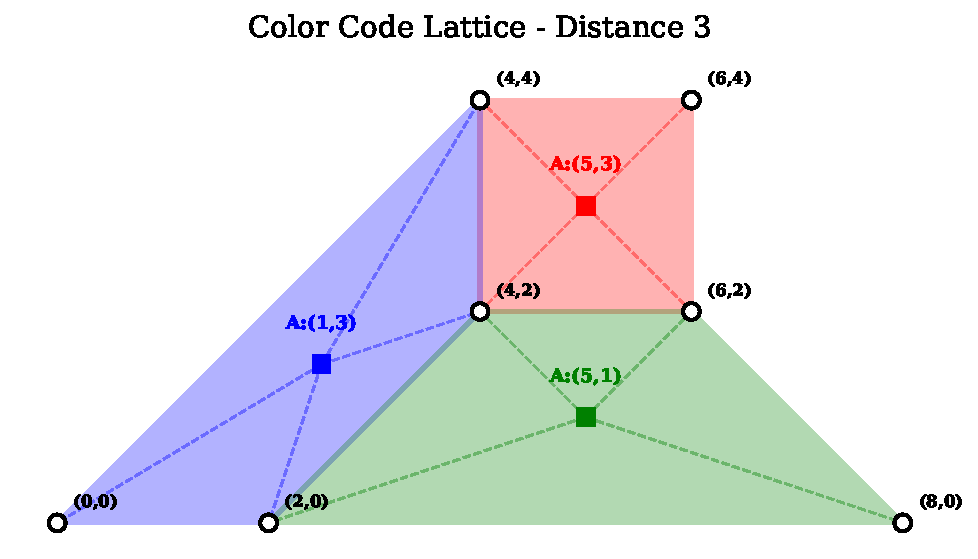
\includegraphics[width=\textwidth]{figures/chapter_6/lattice_d3.pdf}
        \caption{$d=3$}
    \end{subfigure}
    \hfill
    \begin{subfigure}[b]{0.49\textwidth}
        \centering
        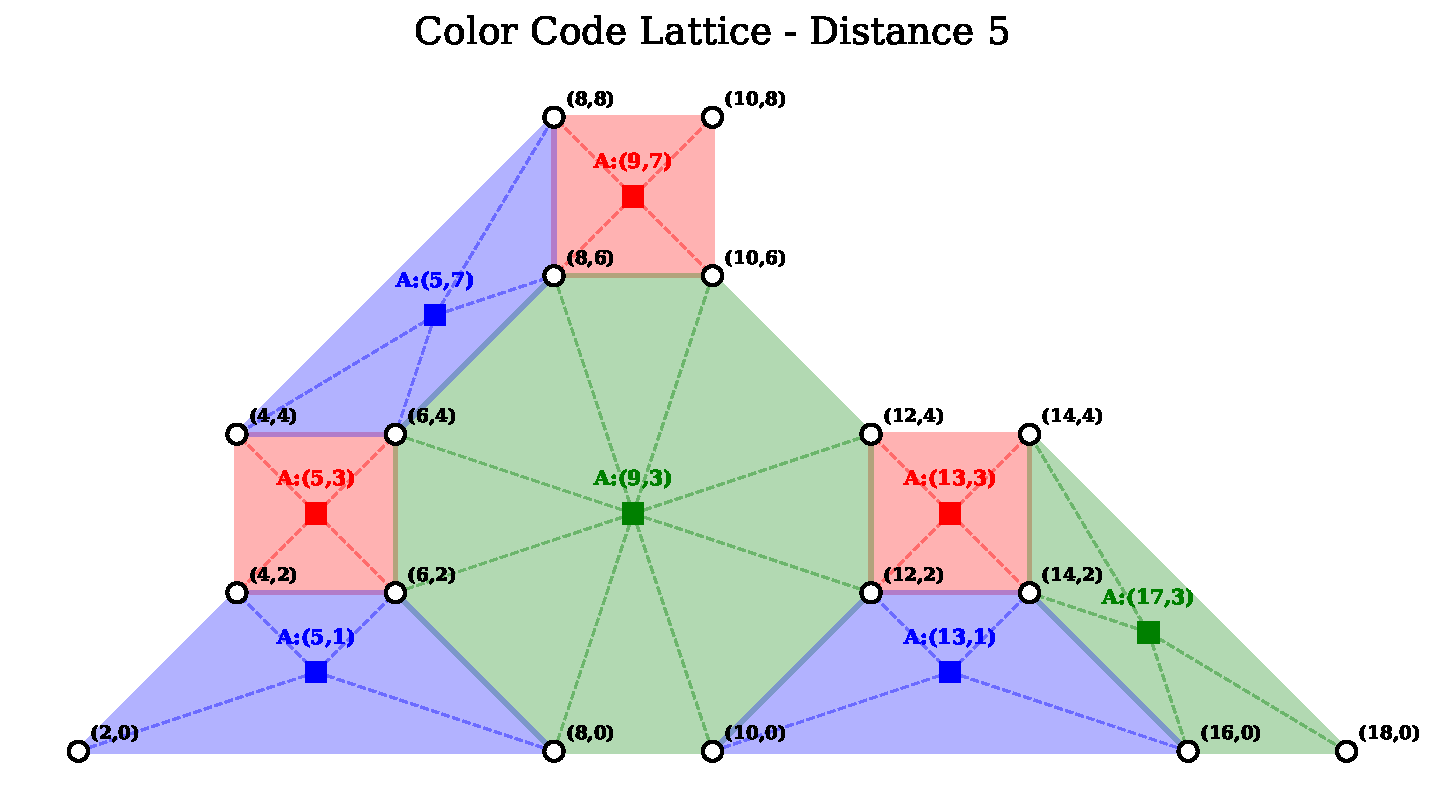
\includegraphics[width=\textwidth]{figures/chapter_6/lattice_d5.pdf}
        \caption{$d=5$}
    \end{subfigure}
    \hfill
    \begin{subfigure}[b]{0.49\textwidth}
        \centering
        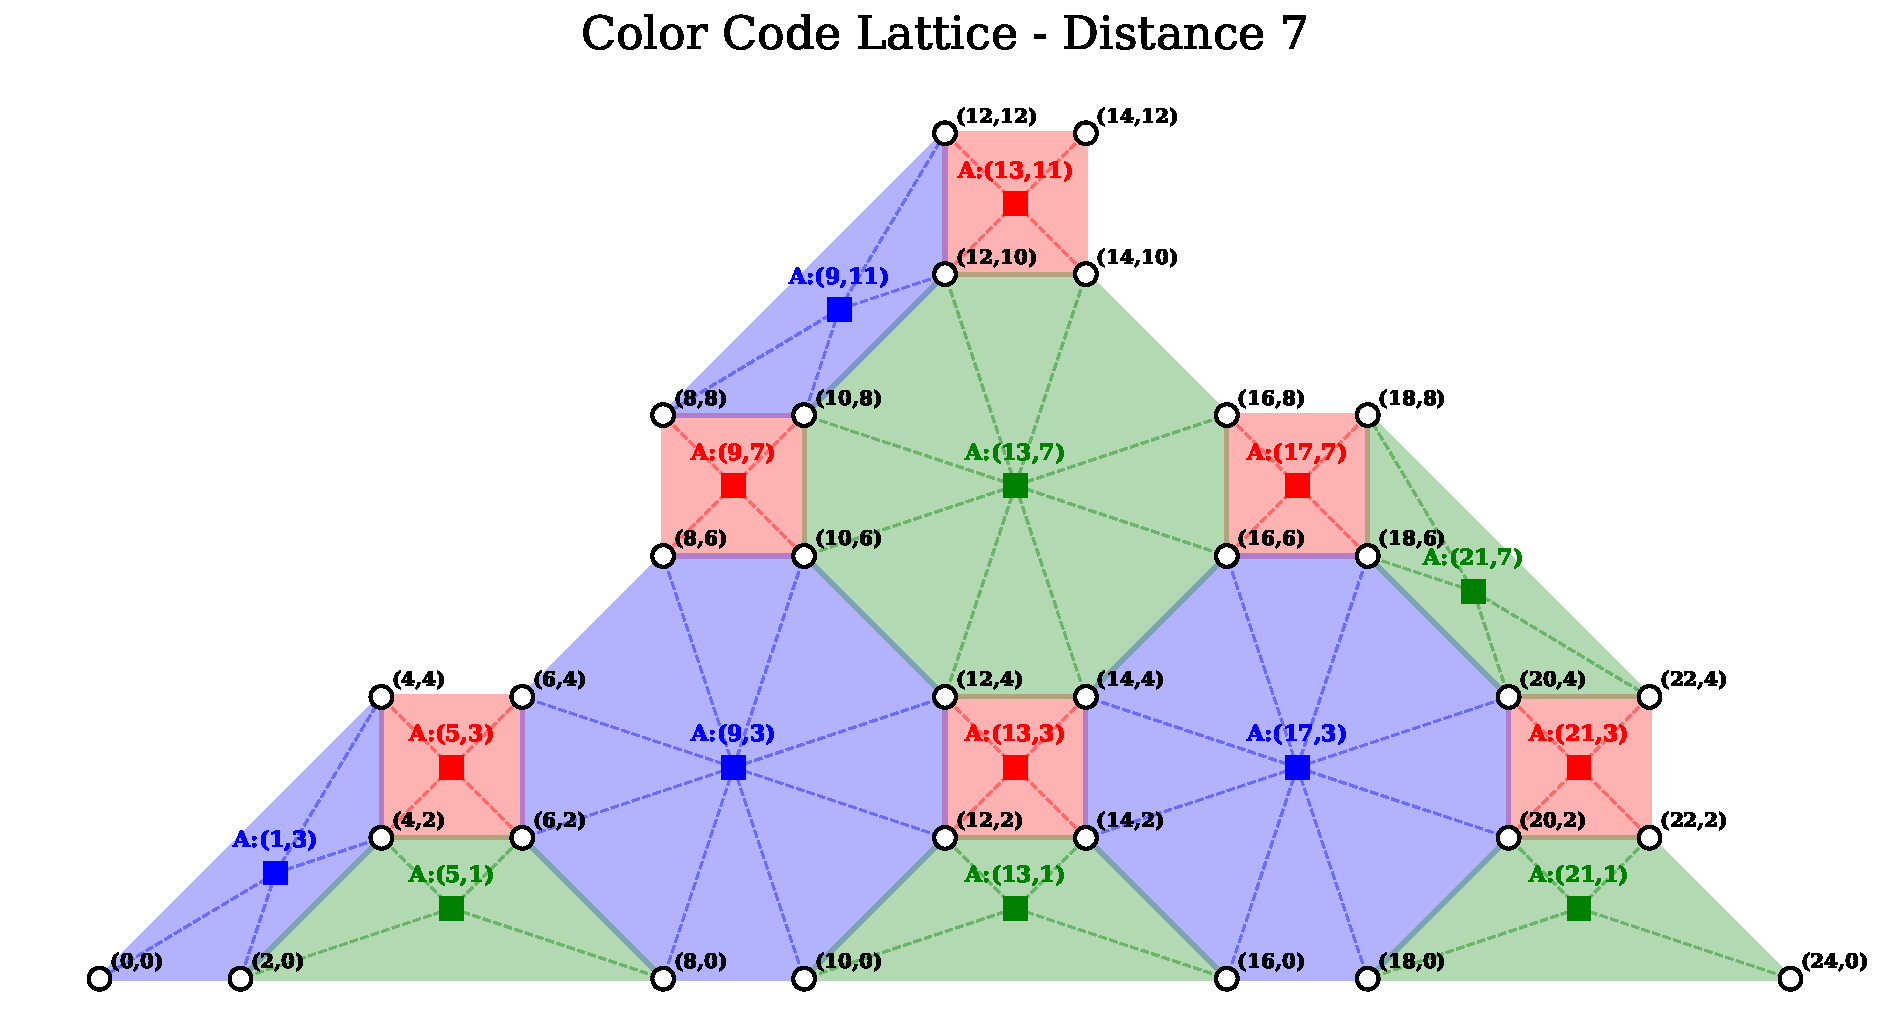
\includegraphics[width=\textwidth]{figures/chapter_6/lattice_d7.pdf}
        \caption{$d=7$}
    \end{subfigure}
    \hfill
    \begin{subfigure}[b]{0.49\textwidth}
        \centering
        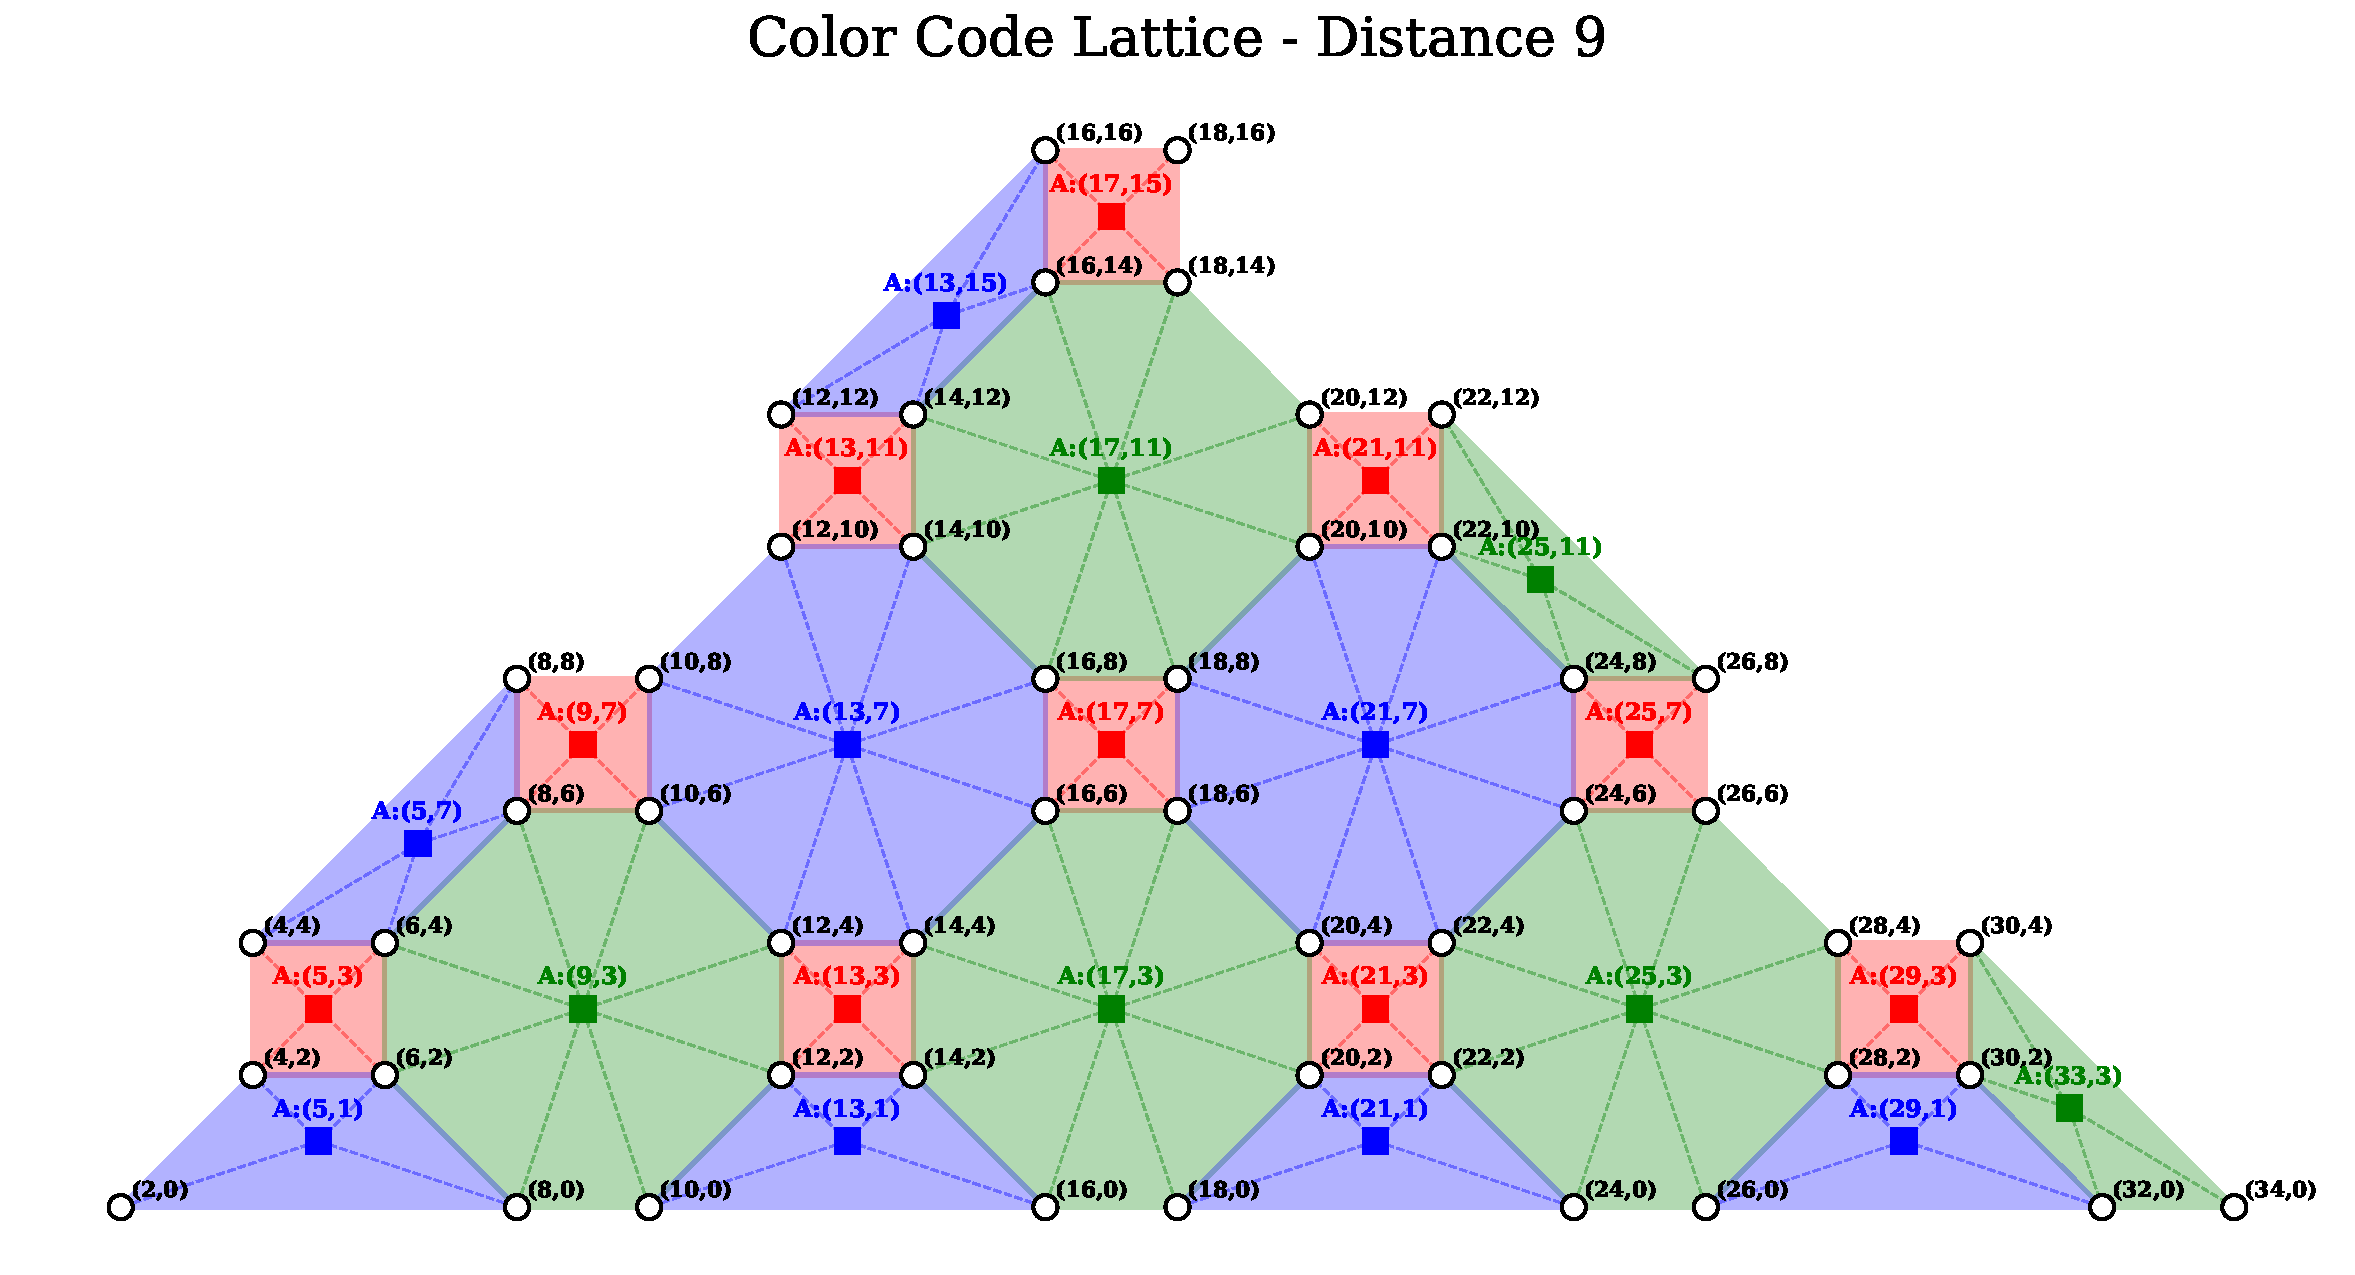
\includegraphics[width=\textwidth]{figures/chapter_6/lattice_d9.pdf}
        \caption{$d=7$}
    \end{subfigure}
    \caption{Evolution of the 4.8.8 Color Code lattice for distances 3, 5, 7 and 9. The solid squares represent the ancilla qubits (syndrome detectors) positioned at the center of each face. The white circles with black outlines represent the physical data qubits. The labels indicate their specific $(x, y)$ coordinates in the simulated grid. High resolution versions of these images are available in the github repository (see Page \pageref{sec:source_code_repository})}
    \label{fig:6:lattice_evolution}
\end{figure}

\subsection{Circuit Generation}
With the geometry resolved, the \texttt{ColorCode} class constructs the quantum circuit. It receives a \texttt{Lattice} object and extracts all unique coordinates, translating them into \texttt{cirq.GridQubit} objects. 

\notatfm{Under a code-capacity error model, the order in which CNOT gates are performed is not relevant. However, under more realistic error models, physical errors can occur during syndrome extraction and propagate through subsequent CNOT gates, causing correlated multi-qubit failures known as \textit{hook errors}. This phenomenon requires a carefully planned CNOT schedule.} Unlike a manual layout, this class dynamically maps the geometric shapes to stabilizer measurement routines. For each syndrome extraction round, it prepares the ancillas, applies Hadamard gates where necessary, and executes CNOT gates between each ancilla and its surrounding data qubits. Finally, it performs a measurement of the data qubits to extract the logical observable.

Detectors are defined after each syndrome extraction. To reduce the number of qubits, ancilla qubits are reused for the $X$ and $Z$ stabilizer measurement, which are sequential. It's worth noting that in the first round $X$ detectors are not added. This is because, with the initial state of the qubits set as $\ket{0}$, measurements in the $X$ axis are not deterministic, so the measured syndrome would be random. After the first round of syndrome measurements, qubit state collapses to a defined value, which can then be used in subsequent rounds to detect phase-flip errors. To allow $Z$ errors to be corrected, we add one initial noiseless round that forces the syndrome to collapse so it can be used later to correct errors.

Similarly, the observable is defined at the end of the circuit. While in the 2D color codes observables are generally defined as a string-nets connecting the boundaries of the lattice (and with minimal weight), an observable defined by all the data qubits is topologically equivalent. This allows us to implement a very simple definition of the observable. 

Figure \ref{fig:6:circuit_d3} illustrates the resulting quantum circuit for a distance 3 code with a single measurement round. 
\begin{figure}[htbp]
    \centering
    \begin{subfigure}[b]{\textwidth}
        \centering
        \begin{adjustbox}{trim=0 0 {0.51\width} 0, clip, max width=\textwidth}
            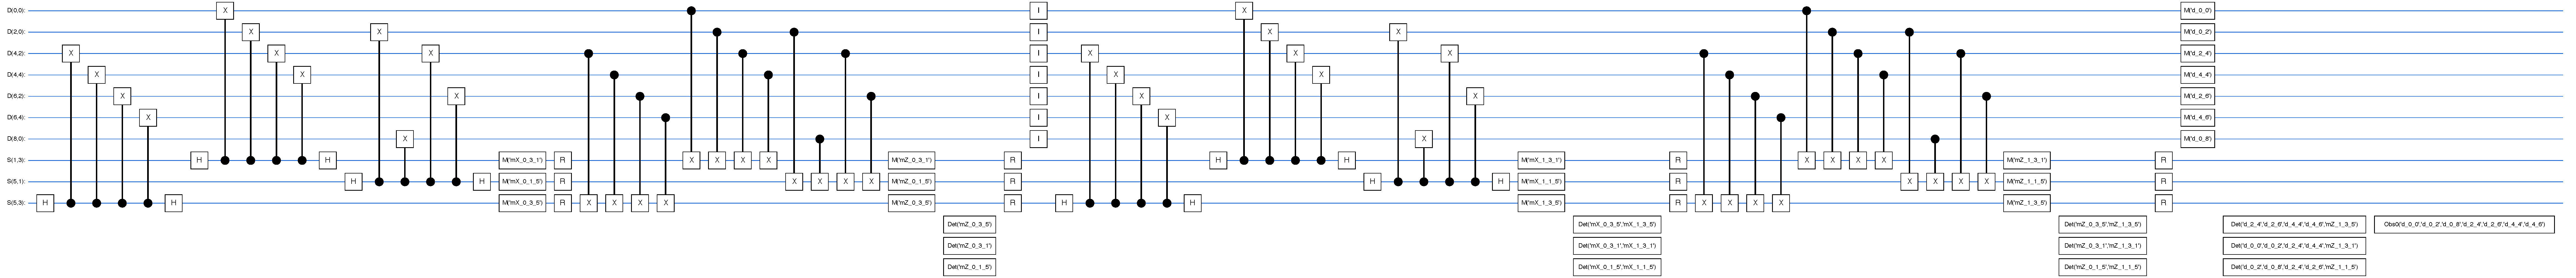
\includegraphics{figures/chapter_6/circuit_d3.pdf}
        \end{adjustbox}
    \end{subfigure}

    \vspace{1ex}
    \begin{subfigure}[b]{\textwidth}
        \centering
        \begin{adjustbox}{trim={0.49\width} 0 0 0, clip, max width=\textwidth}
            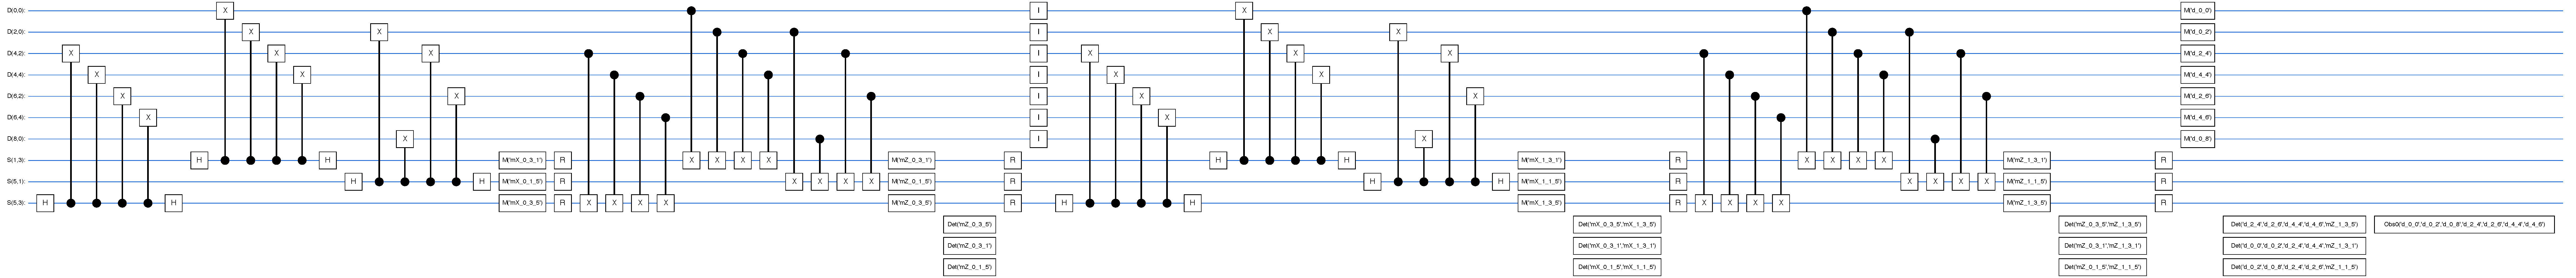
\includegraphics{figures/chapter_6/circuit_d3.pdf}
        \end{adjustbox}
    \end{subfigure}
    \caption{Complete quantum circuit for the 4.8.8 Color Code ($d=3$, 1 round). The data qubits have been labeled as $D(x,y)$ and the ancilla qubits for the stabilizers as $S(x,y)$, so they are grouped to ease the visualization. Due to its significant width, the image has been dynamically split into two halves for readability. High resolution versions of these images are available in the github repository (see Page \pageref{sec:source_code_repository})}
    \label{fig:6:circuit_d3}
\end{figure}

\section{Simulation Architecture and Evaluation Metrics}
\label{sec:simulation_architecture}

To systematically evaluate and compare the performance of different decoders on the 2D Color Code, it is essential to establish a robust, automated, and scalable simulation pipeline. Rather than writing isolated scripts for each decoding algorithm, we have designed a unified modular architecture that leverages the \texttt{sinter} library described in Chapter \ref{chap:implementation_and_simulation}.

The architecture is composed of three main intercommunicating modules:

\begin{enumerate}
    \item \textbf{The simulation manager (\texttt{simulator.py}):} This is the main entry point for a given simulation. It receives a configuration matrix detailing the code distances ($d$) and the physical error rates ($p$) to simulate. For each configuration, it invokes the \texttt{ColorCode} generator (discussed in Section~\ref{sec:implementation_color_code}) to dynamically create the Stim circuits and the corresponding Detector Error Models (DEM). Because generating these symbolic models can be computationally expensive, the simulator implements a caching system. It saves the \texttt{.stim} and \texttt{.dem} files to disk, automatically detecting when parameters change to invalidate and clean the cache, speeding up subsequent runs.
    
    \item \textbf{The decoder interface (\texttt{decoder\_interfaces.py}):} To ensure the simulation pipeline works similarly with any decoding algorithm being tested, all decoders are wrapped into \texttt{sinter.Decoder}, which is an adapter class. This module acts as a plug-and-play interface that standardizes the input (syndrome data) and the output (logical predictions), allowing us to swap the decoder with a single parameter change.
    
    \item \textbf{Data storage and visualization (\texttt{plotter.py}):} As \texttt{sinter} processes the shots, the raw statistical results (total shots, logical errors observed, and execution time) are systematically appended to a CSV file, so the data can be used and compared later, which will be critical in Chapter \ref{chap:comparative_analysis}. Once the simulation concludes, the CSV data is plotted and stored. At this stage, we also perform an interpolation of the logical error rate curves to determine their crossing points, and average all the crossing points to estimate the threshold $p_{th}$.
\end{enumerate}

\notatfm{Tracking the execution time is key to later evaluate the empirical computational complexity of each algorithm, which determines whether a decoder can keep up with the physical quantum hardware speeds.} By structuring the project this way, we can guarantee that all algorithms are subjected to the exact same conditions. The captured data allows measuring the four key metrics that will drive the comparative analysis:

\begin{itemize}
    \item \textbf{Determination of error thresholds ($p_{th}$):} Identifying the crossing point in the logical error curves where increasing the code distance begins to suppress errors rather than amplifying them.
    \item \textbf{Logical failure rate ($p_L$) scaling as a function of physical error rate ($p$) and code distance ($d$):} Analyzing the curves to evaluate the decoder's raw accuracy.
    \item \textbf{Sub-threshold scaling analysis and theoretical suppression limits:} Evaluating how steeply the logical error drops when operating below the threshold.
    \item \textbf{Computational complexity and empirical decoding time (Accuracy vs. Speed trade-off):} Analyzing the empirical decoding time to determine if the decoder's complexity is practically scalable.
\end{itemize}

With this systematic architecture in place, we are now ready to implement and simulate the specific decoding algorithms.



\section{BP+OSD}
\label{sec:6:bposd}

As discussed in Chapter \ref{chap:qec_decoders}, the Belief Propagation with Ordered Statistics Decoding (BP+OSD) algorithm provides a method to decode 2D Color Codes without projections or other adaptations. However, this flexibility comes at the cost of higher complexity. The BP+OSD algorithm allows several parameters to fine-tune its performance and complexity. 

In this section, we first perform a systematic optimization of these parameters to identify the optimal configuration for our specific 4.8.8 lattice geometry. Subsequently, we use the optimized decoder to execute a full threshold evaluation.

\subsection{Parameter Optimization}
\label{subsec:6:bposd_optimization}

To isolate the effect of the different BP+OSD parameters, we fixed the lattice distance to $d=7$ and evaluated the decoder's performance across a range of physical depolarizing error rates. Our optimization focuses on three key components: the BP update rule, the OSD method, and the OSD search order.

\subsubsection{BP Update Rule Comparison}
The standard Belief Propagation algorithm utilizes the Product-Sum (PS) update rule, which computes exact probabilities. A widely used alternative is the Min-Sum (MS) approximation, which simplifies the check-node updates. This minimizes computational overhead and can mitigate the effect of the short cycles present in the color code Tanner graph.

Figure \ref{fig:6:bposd_bp_methods} compares both approaches. The empirical results show that the Min-Sum and Product-Sum rules yield virtually identical logical error rates. However, the Min-Sum approximation consistently reduces the average execution time. Based on these results, we select the Min-Sum (MS) update rule to accelerate all subsequent simulations.

\begin{figure}[htbp]
    \centering
    \begin{subfigure}[b]{0.49\textwidth}
        \centering
        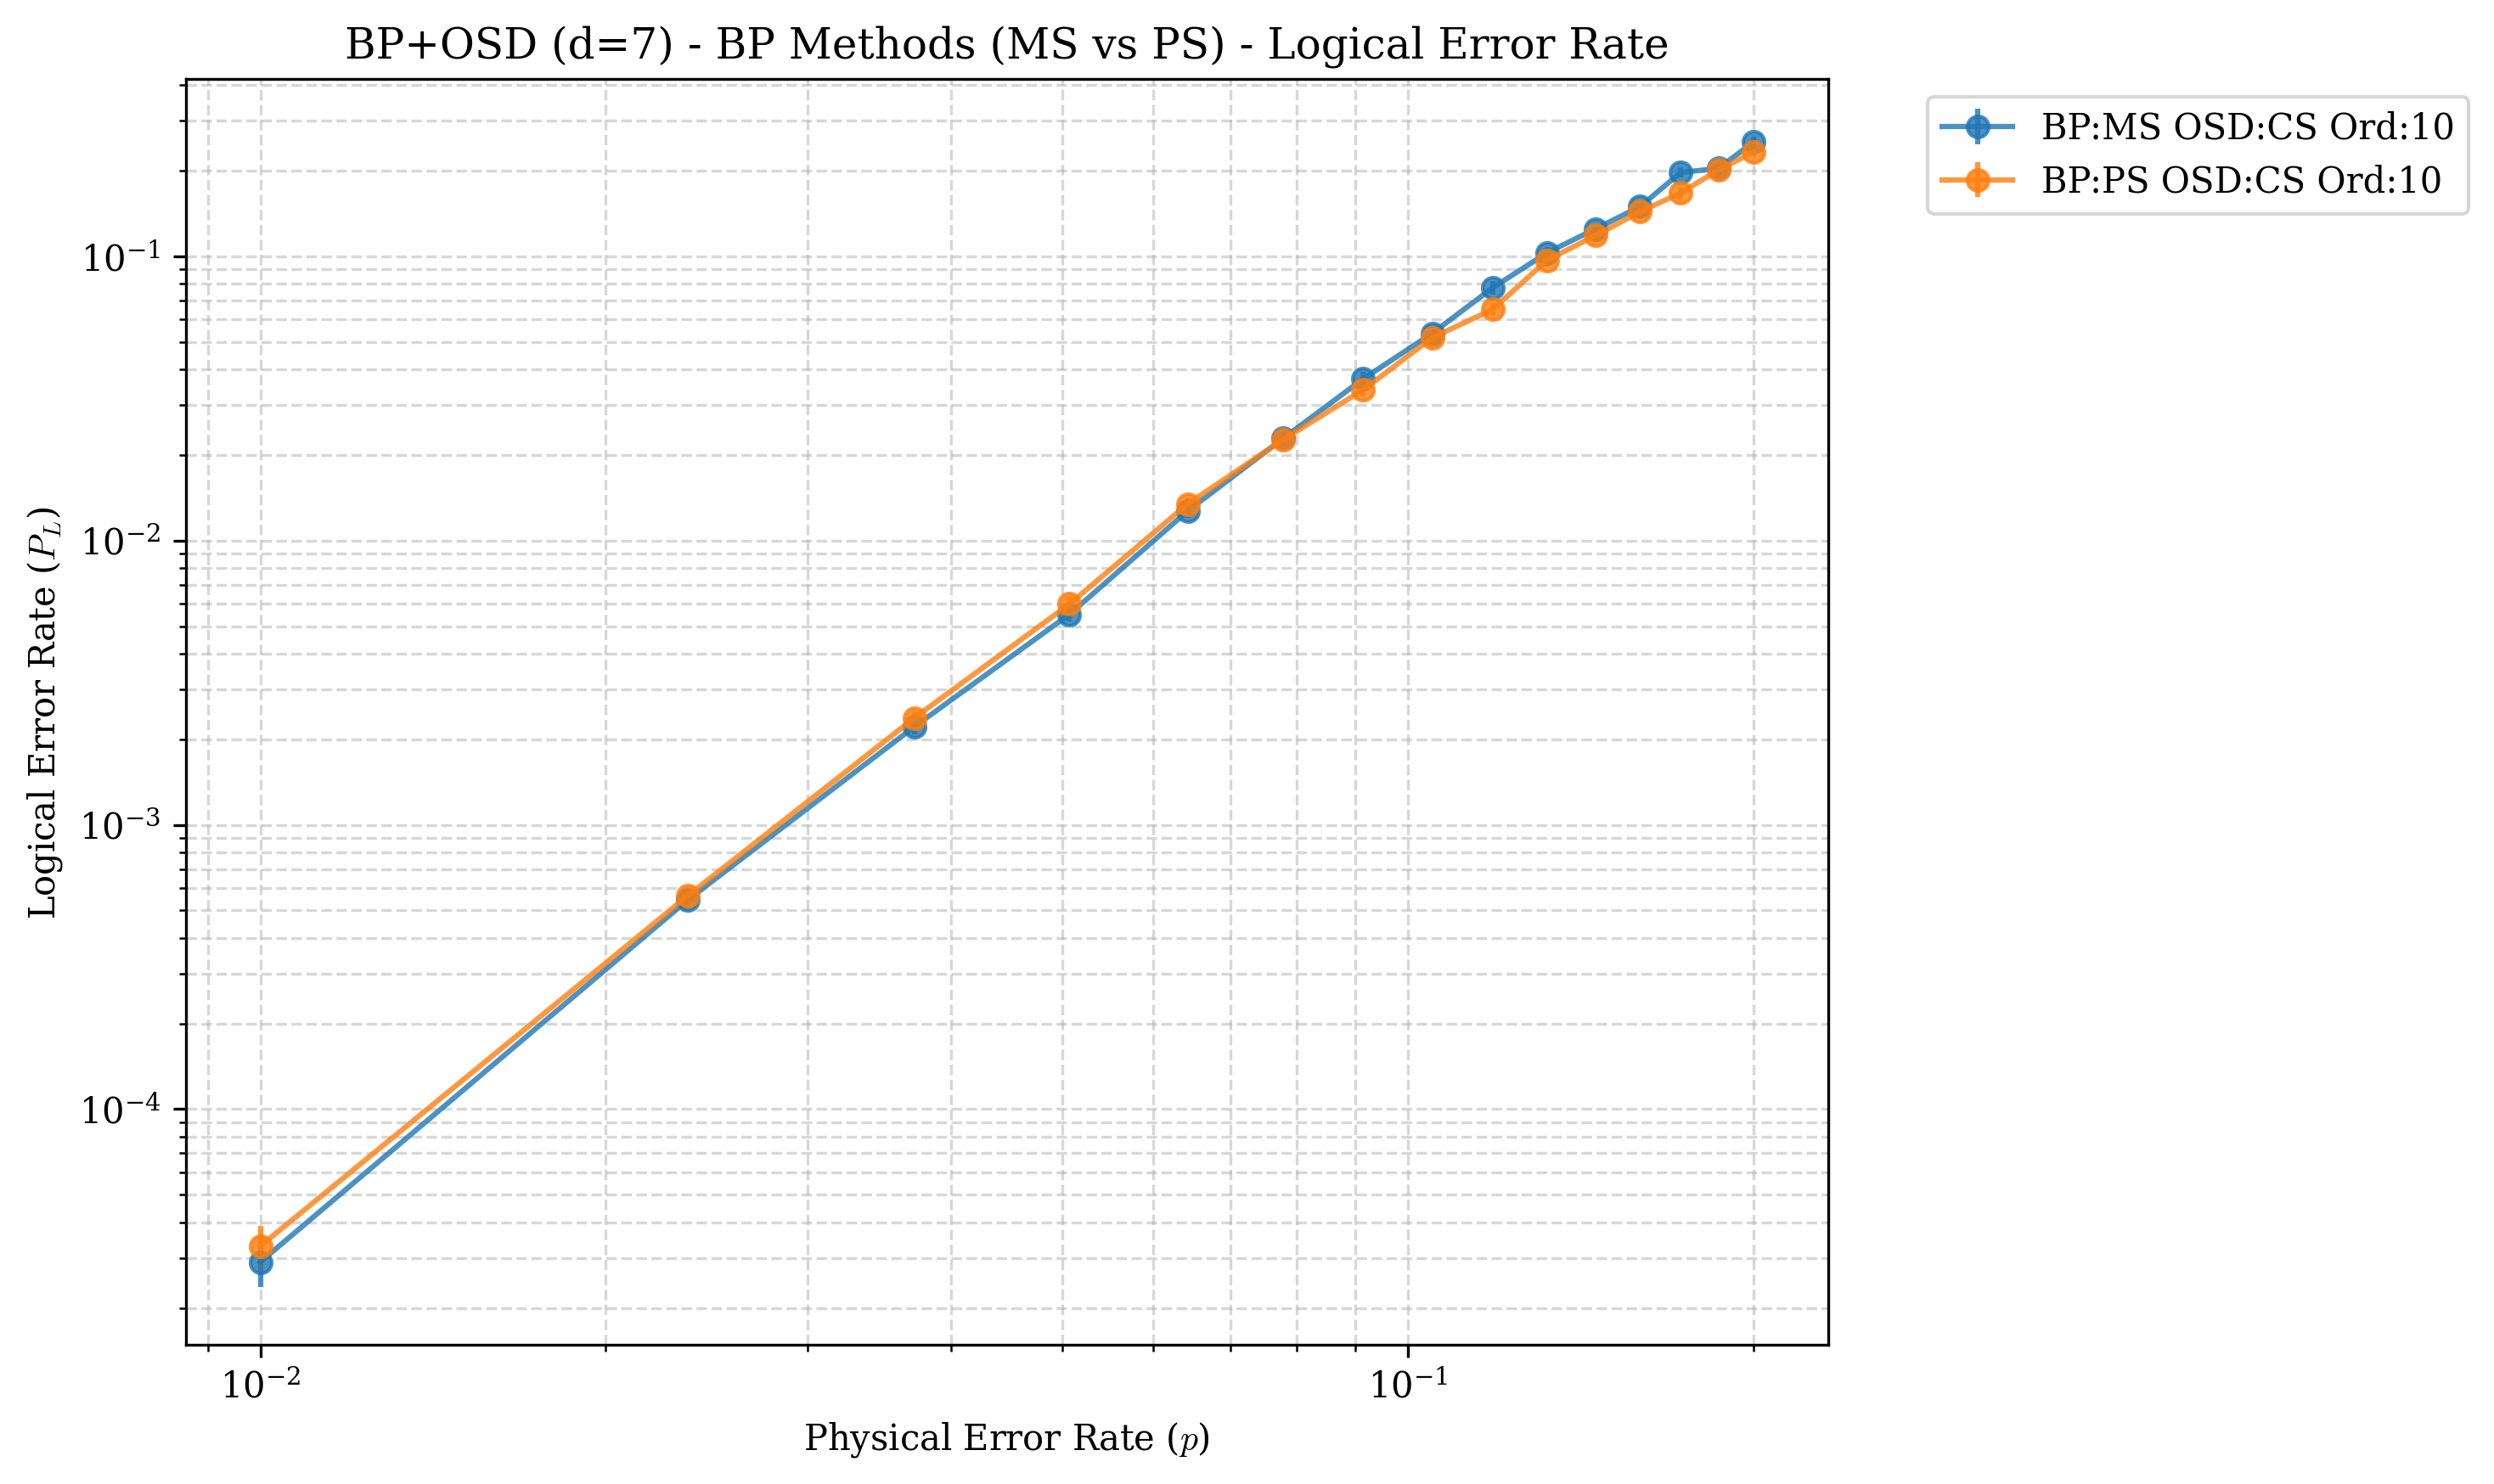
\includegraphics[width=\textwidth]{figures/chapter_6/s2b_bposd_bp_methods_error.png}
    \end{subfigure}
    \hfill
    \begin{subfigure}[b]{0.49\textwidth}
        \centering
        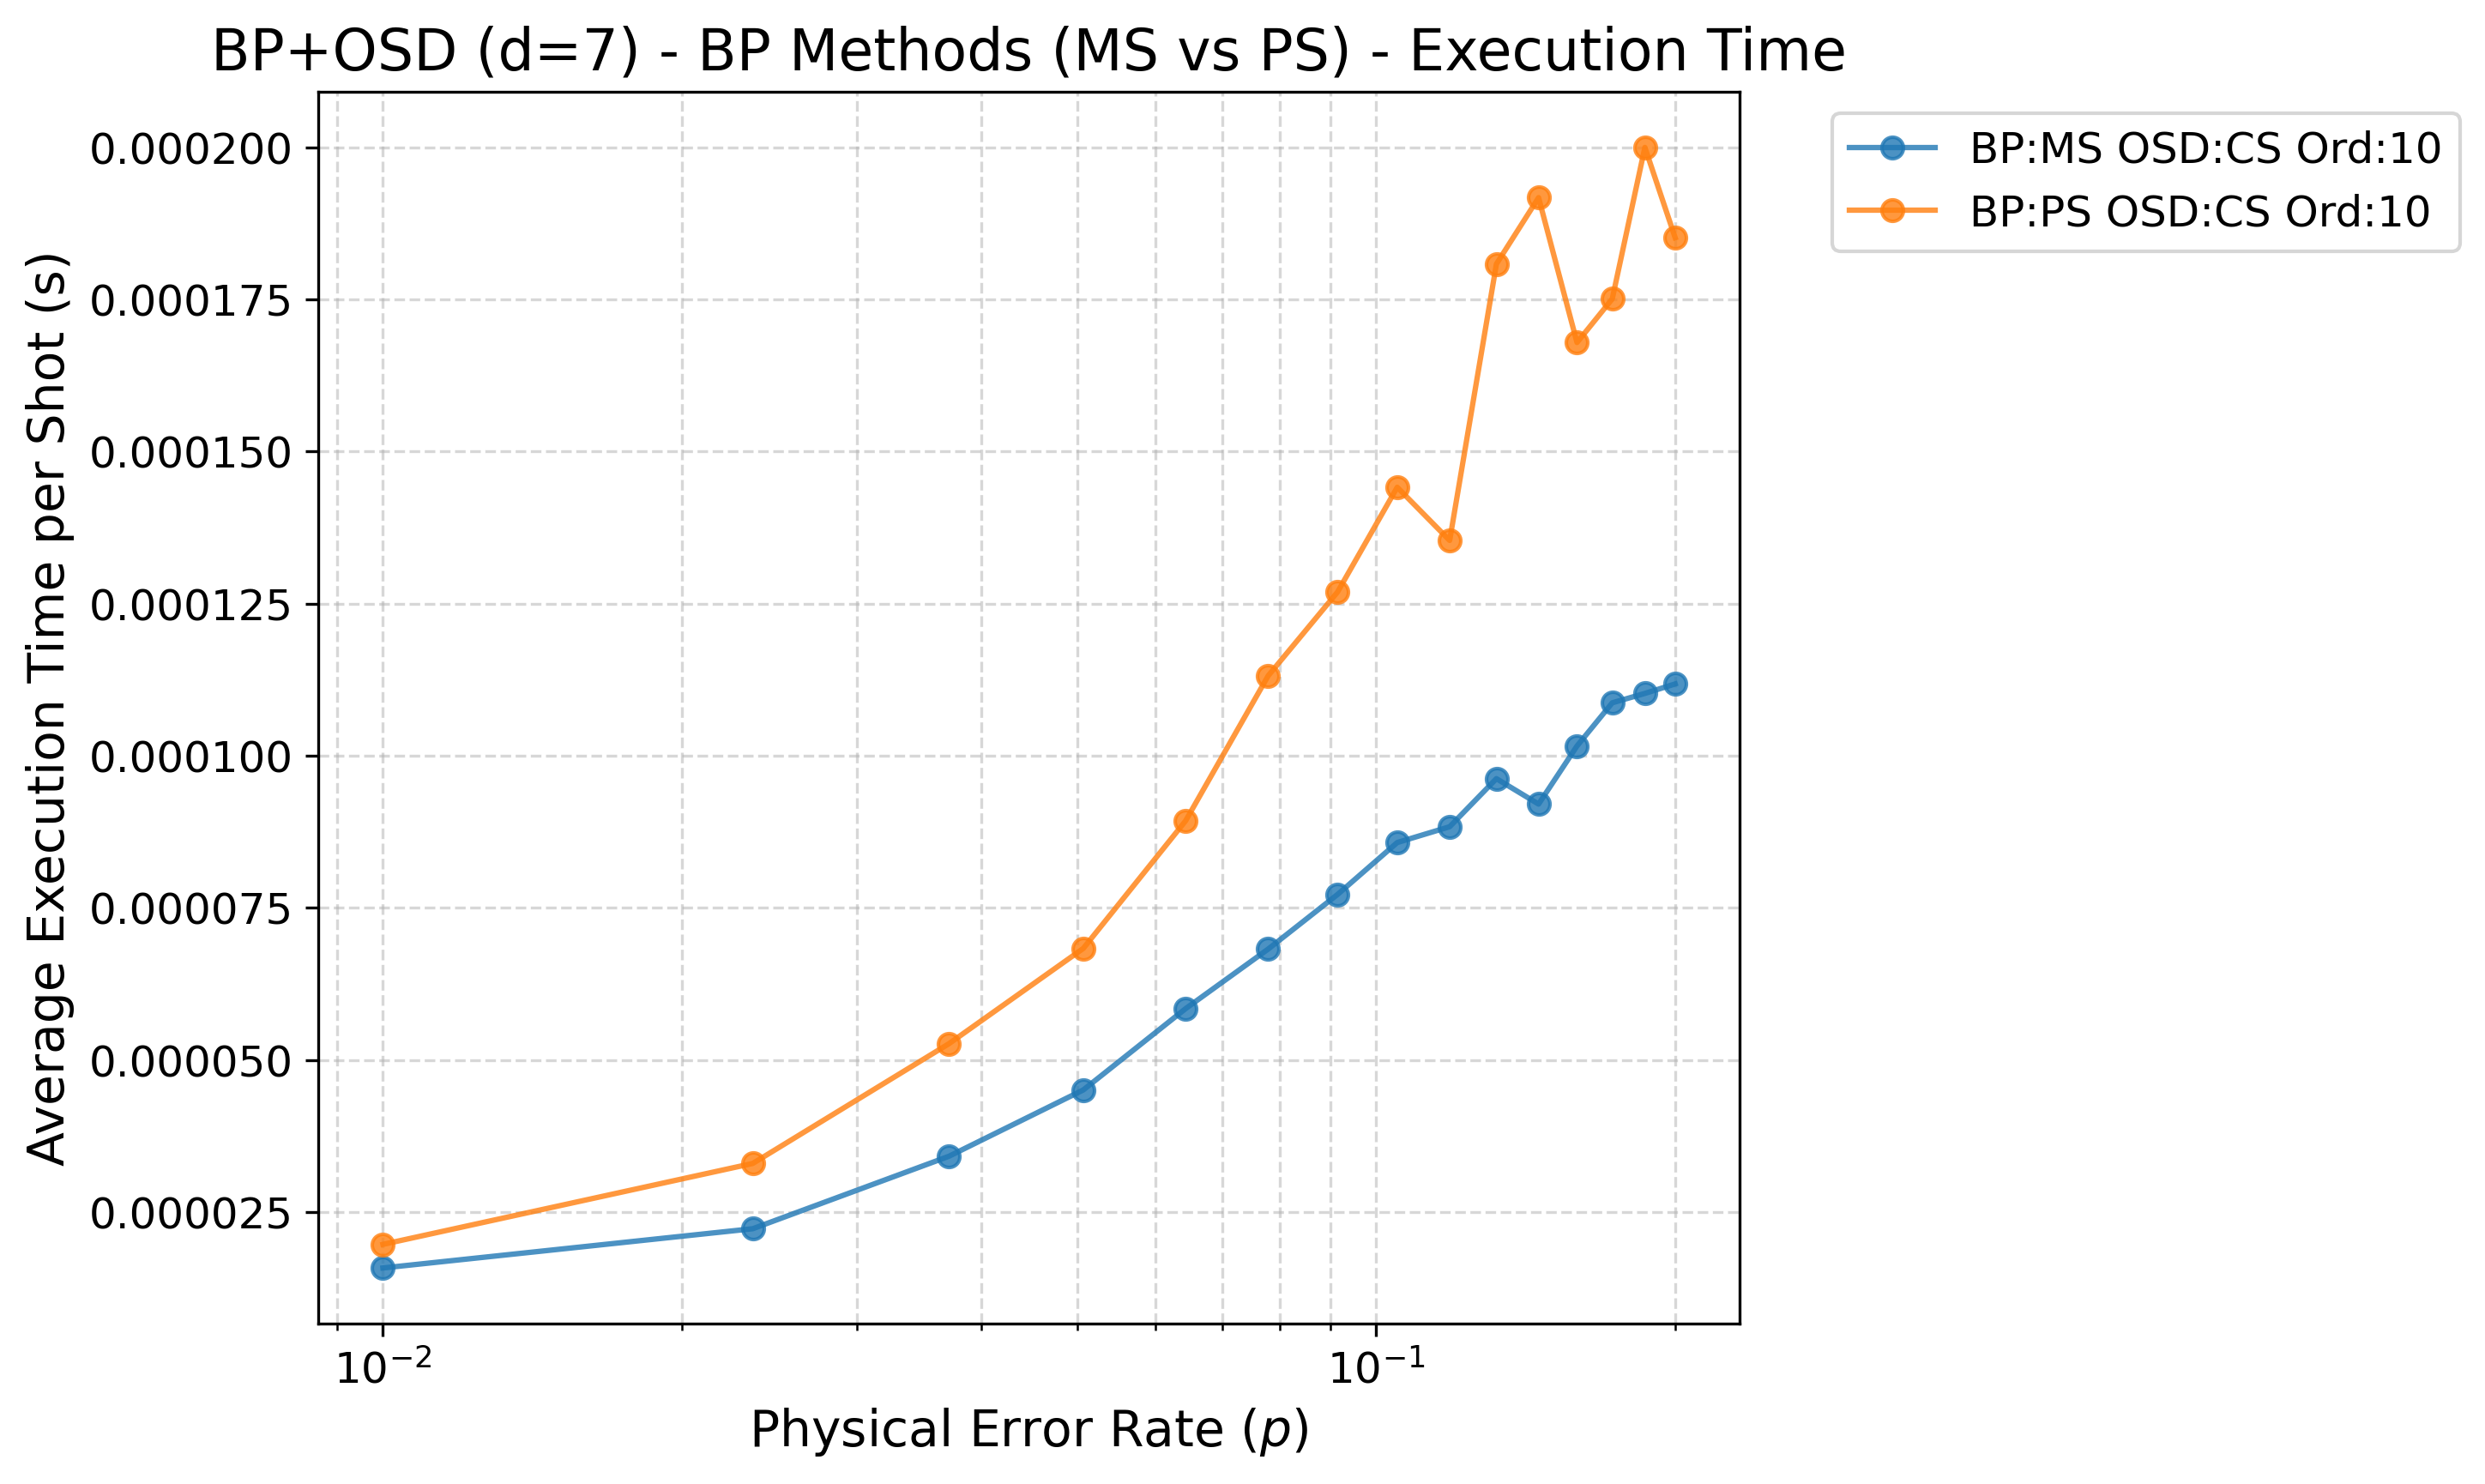
\includegraphics[width=\textwidth]{figures/chapter_6/s2b_bposd_bp_methods_time.png}
    \end{subfigure}
    \caption{Performance comparison of the Min-Sum and Product-Sum BP update rules for $d=7$. The logical error rate (left) remains largely unaffected, but the Min-Sum approximation provides a clear advantage in execution time (right).}
    \label{fig:6:bposd_bp_methods}
\end{figure}

\subsubsection{OSD Method Comparison}
When BP fails to converge, the OSD post-processing phase forces a valid solution based on the soft probabilities. We evaluated three OSD strategies, maintaining a constant search order of $k=5$ when applicable:
\begin{itemize}
    \item \textbf{Order-0 (\texttt{osd\_0}):} Directly applies Gaussian elimination without further search.
    \item \textbf{Exhaustive (\texttt{osd\_e}):} Performs an exhaustive search over the $k$ least reliable qubits.
    \item \textbf{Combination Sweep (\texttt{osd\_cs}):} Explores a wider non exhaustive search over the least reliable qubits, with $k$ controlling the search depth.
\end{itemize}

\notatfm{While \texttt{osd\_e} is an exhaustive search, it is limited to the $k$ lowest-confidence qubits, which prevents it from evaluating highly probable error combinations that include other qubits. \texttt{osd\_cs} overcomes this by sampling combinations across a wider subset of uncertain qubits.} As depicted in Figure \ref{fig:6:bposd_osd_methods}, \texttt{osd\_0} underperforms significantly because it entirely trusts the unconverged BP probabilities. The Exhaustive method (\texttt{osd\_e}) improves the threshold, but the Combination Sweep method (\texttt{osd\_cs}) heavily outperforms both by efficiently exploring combinations of likely error vectors. Consequently, \texttt{osd\_cs} is selected as our baseline OSD method.

\begin{figure}[htbp]
    \centering
    \begin{subfigure}[b]{0.49\textwidth}
        \centering
        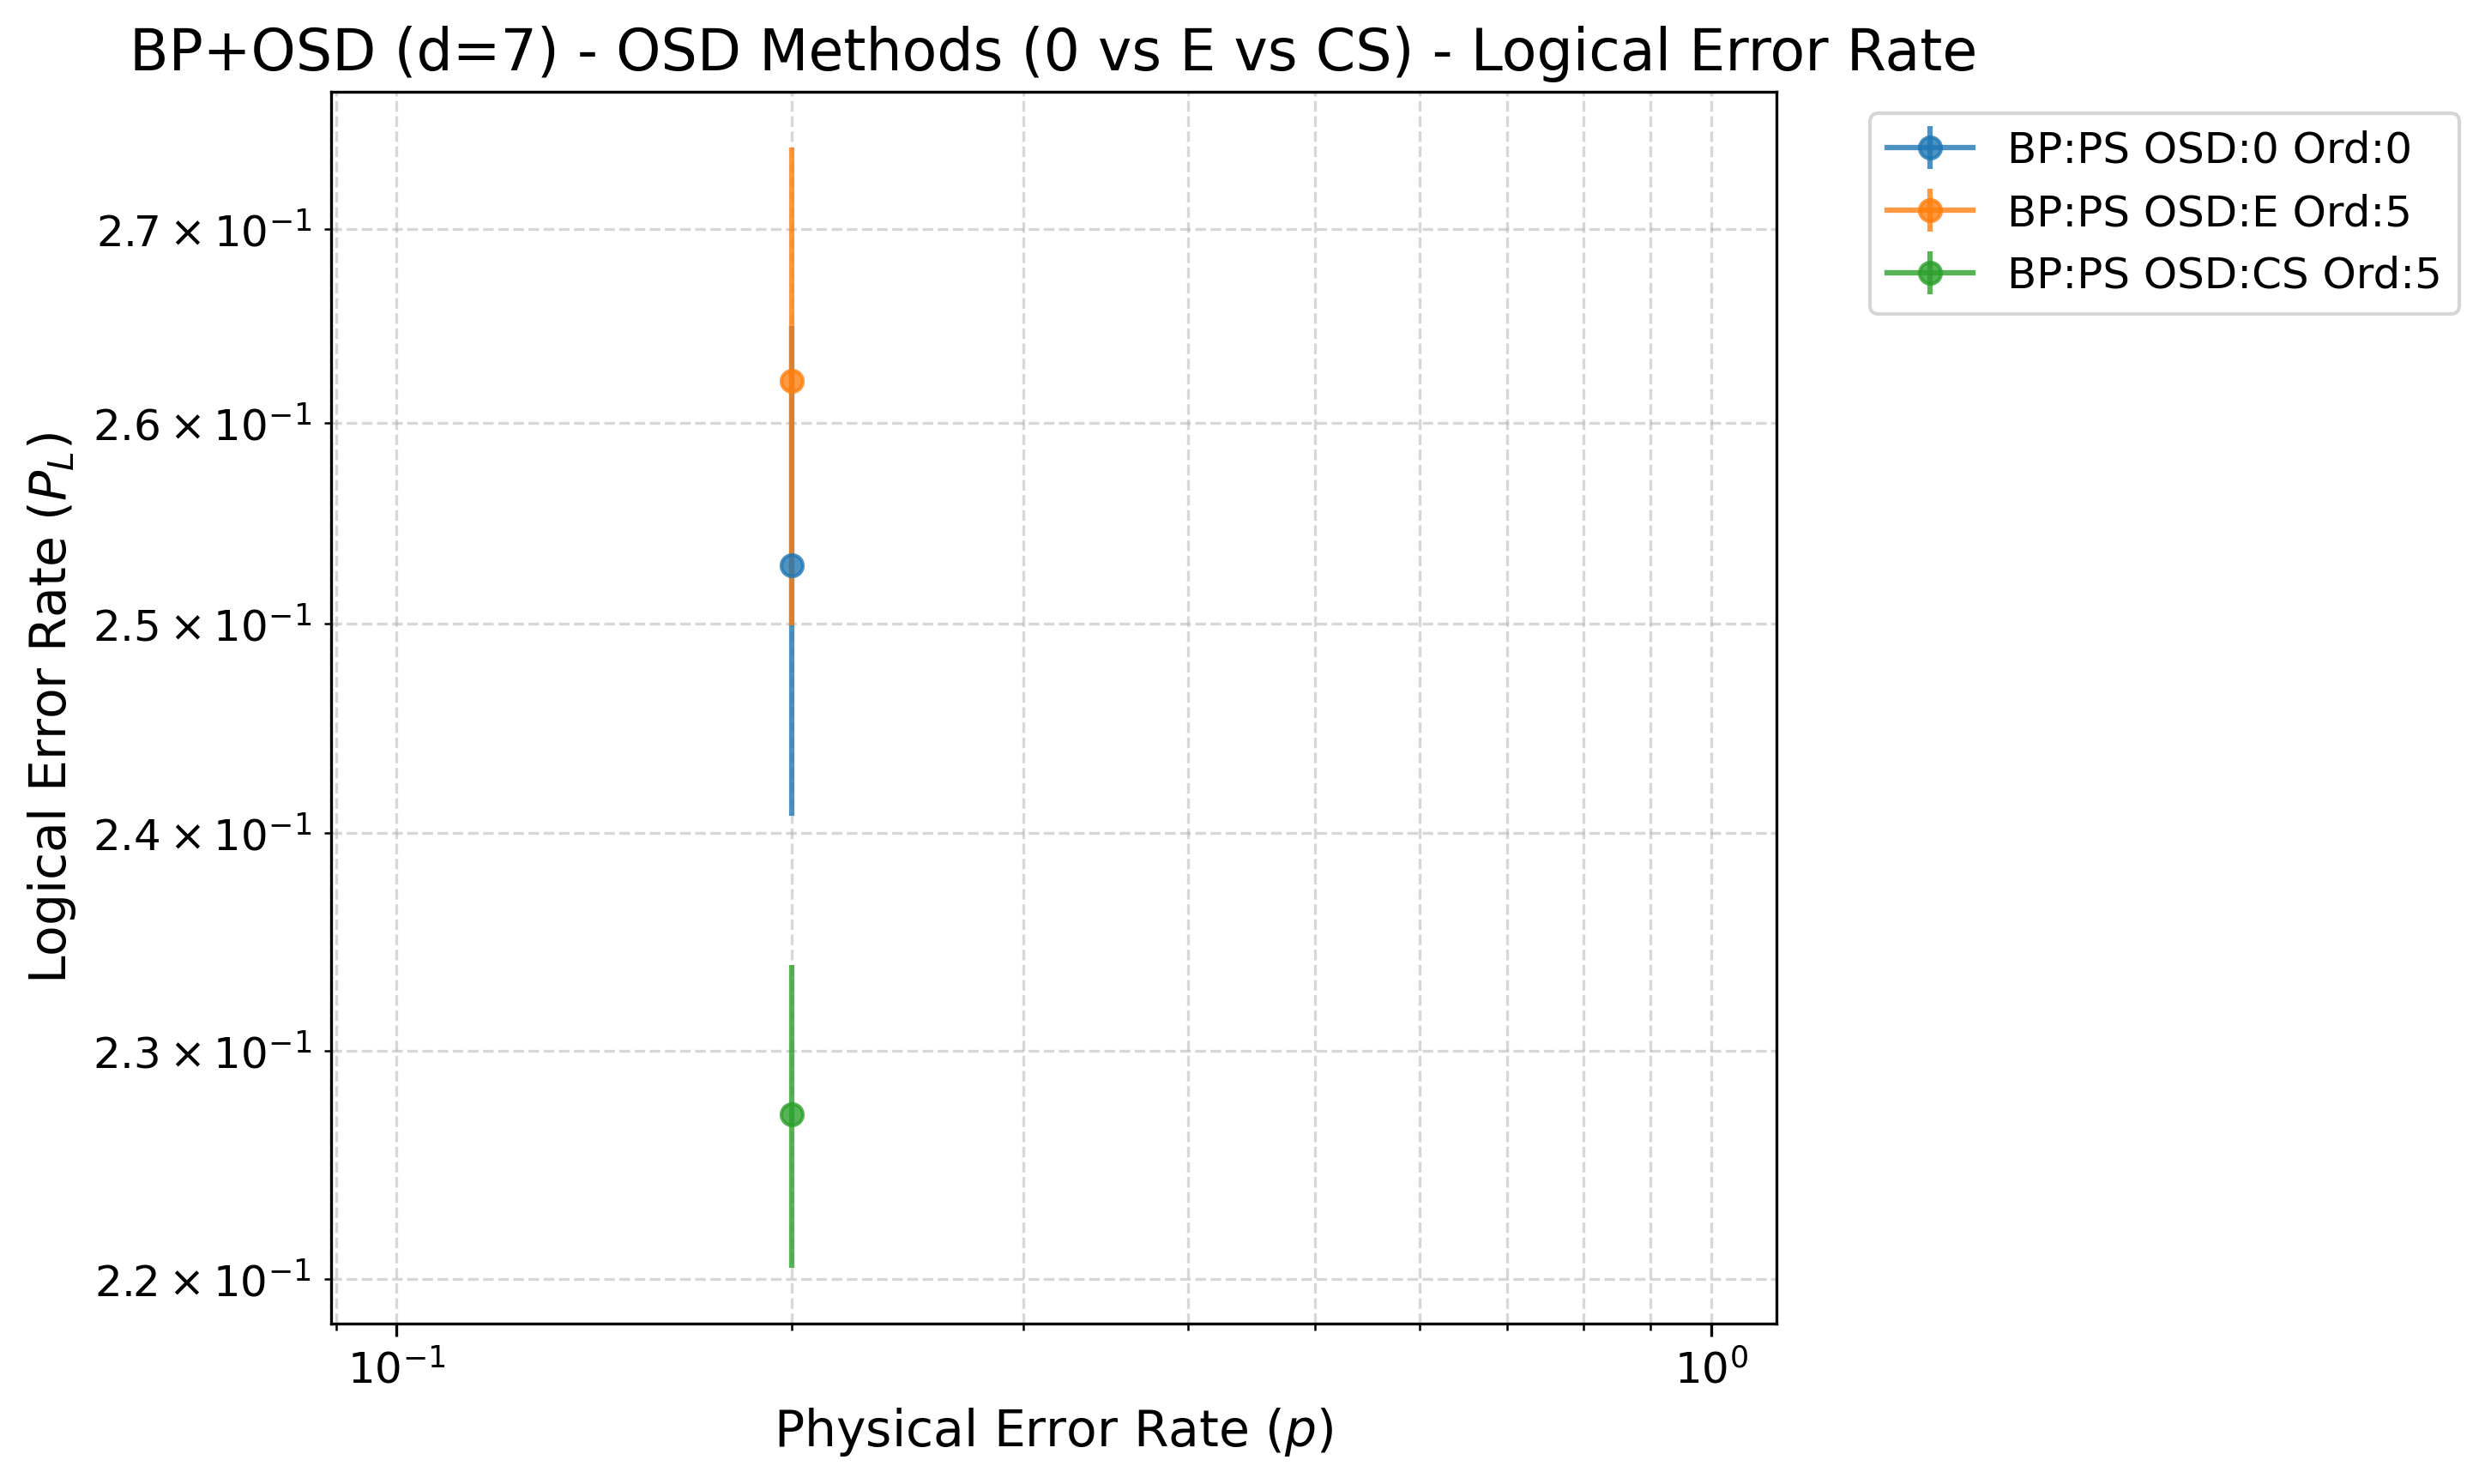
\includegraphics[width=\textwidth]{figures/chapter_6/s2b_bposd_osd_methods_error.png}
    \end{subfigure}
    \hfill
    \begin{subfigure}[b]{0.49\textwidth}
        \centering
        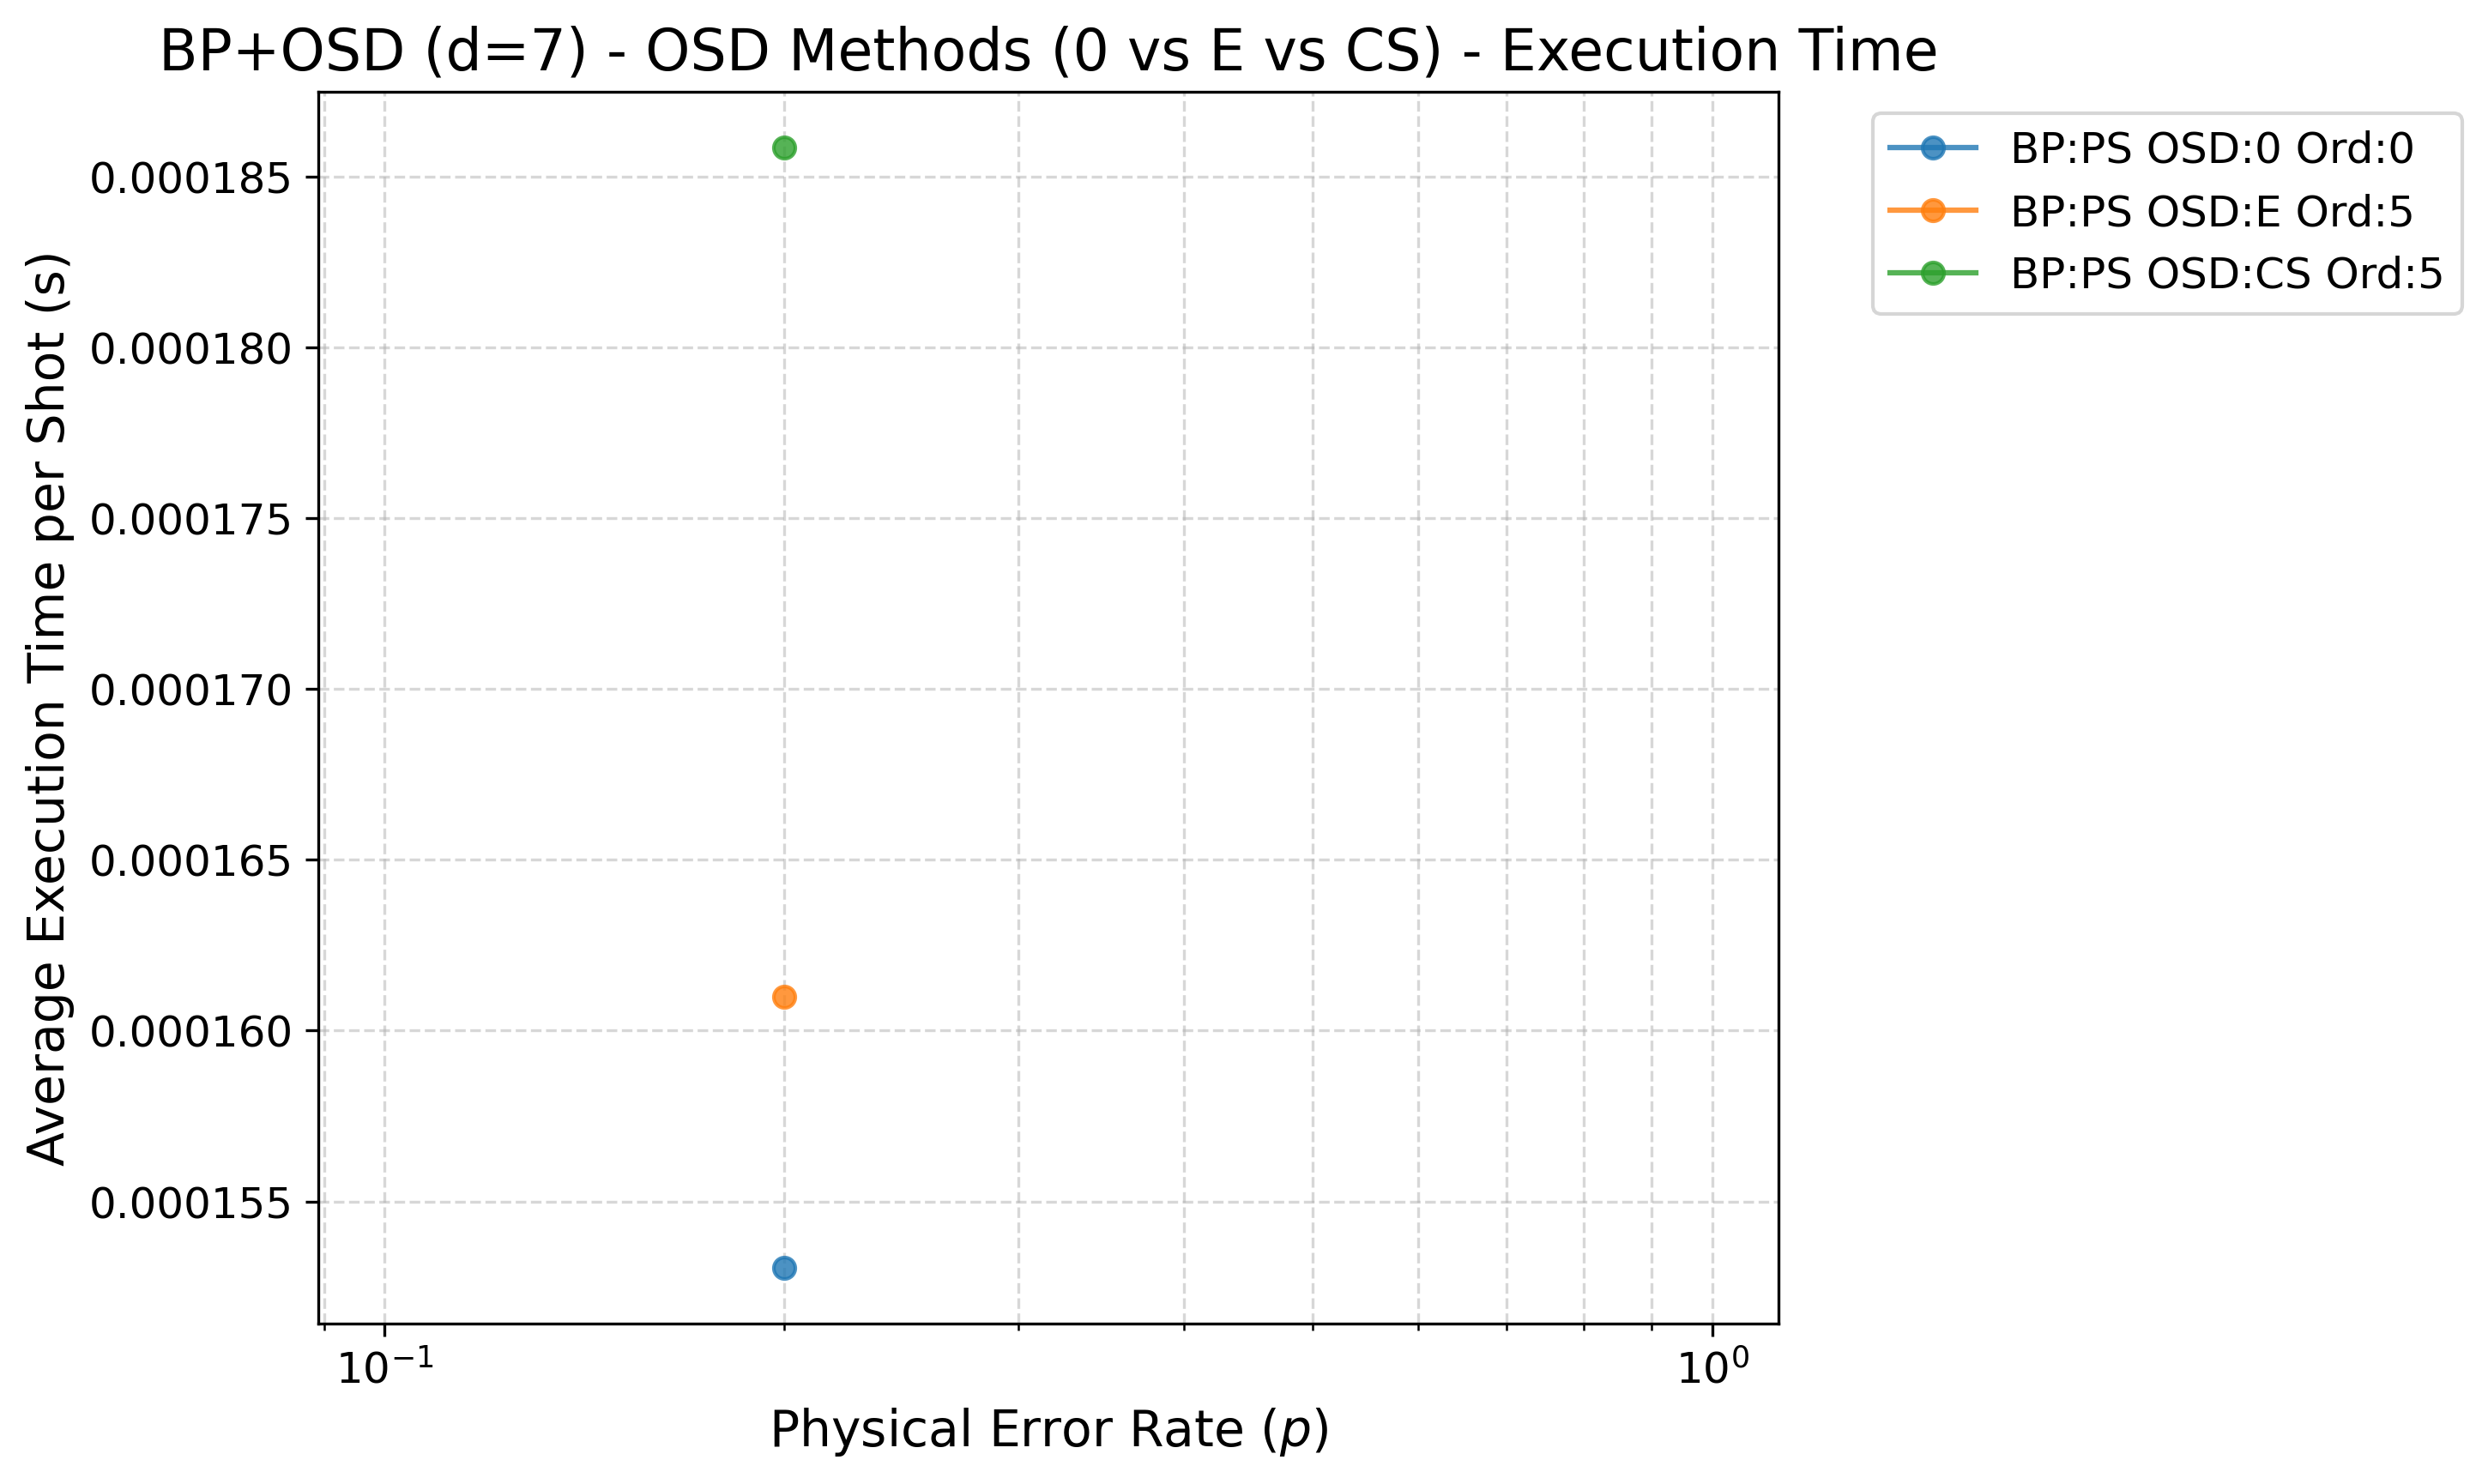
\includegraphics[width=\textwidth]{figures/chapter_6/s2b_bposd_osd_methods_time.png}
    \end{subfigure}
    \caption{Comparison of different OSD post-processing strategies (\texttt{osd\_0}, \texttt{osd\_e}, \texttt{osd\_cs}) at a fixed search order $k=5$. The Combination Sweep method yields the lowest logical error rates.}
    \label{fig:6:bposd_osd_methods}
\end{figure}

\subsubsection{OSD Search Order Analysis}
Having selected \texttt{osd\_cs}, we must define its search order $k$. A higher order allows the decoder to explore more alternative hypotheses, improving accuracy but heavily penalizing execution time due to the combinatorial explosion.

Figure \ref{fig:6:bposd_osd_orders} illustrates this trade-off. Increasing $k$ from 5 to 10 yields a notable improvement in the logical error rate. However, pushing $k$ to 20 provides highly diminishing returns while severely impacting the execution speed. To maintain computational feasibility without significantly sacrificing the decoding threshold, we fix the OSD order at $k=10$.

\begin{figure}[htbp]
    \centering
    \begin{subfigure}[b]{0.49\textwidth}
        \centering
        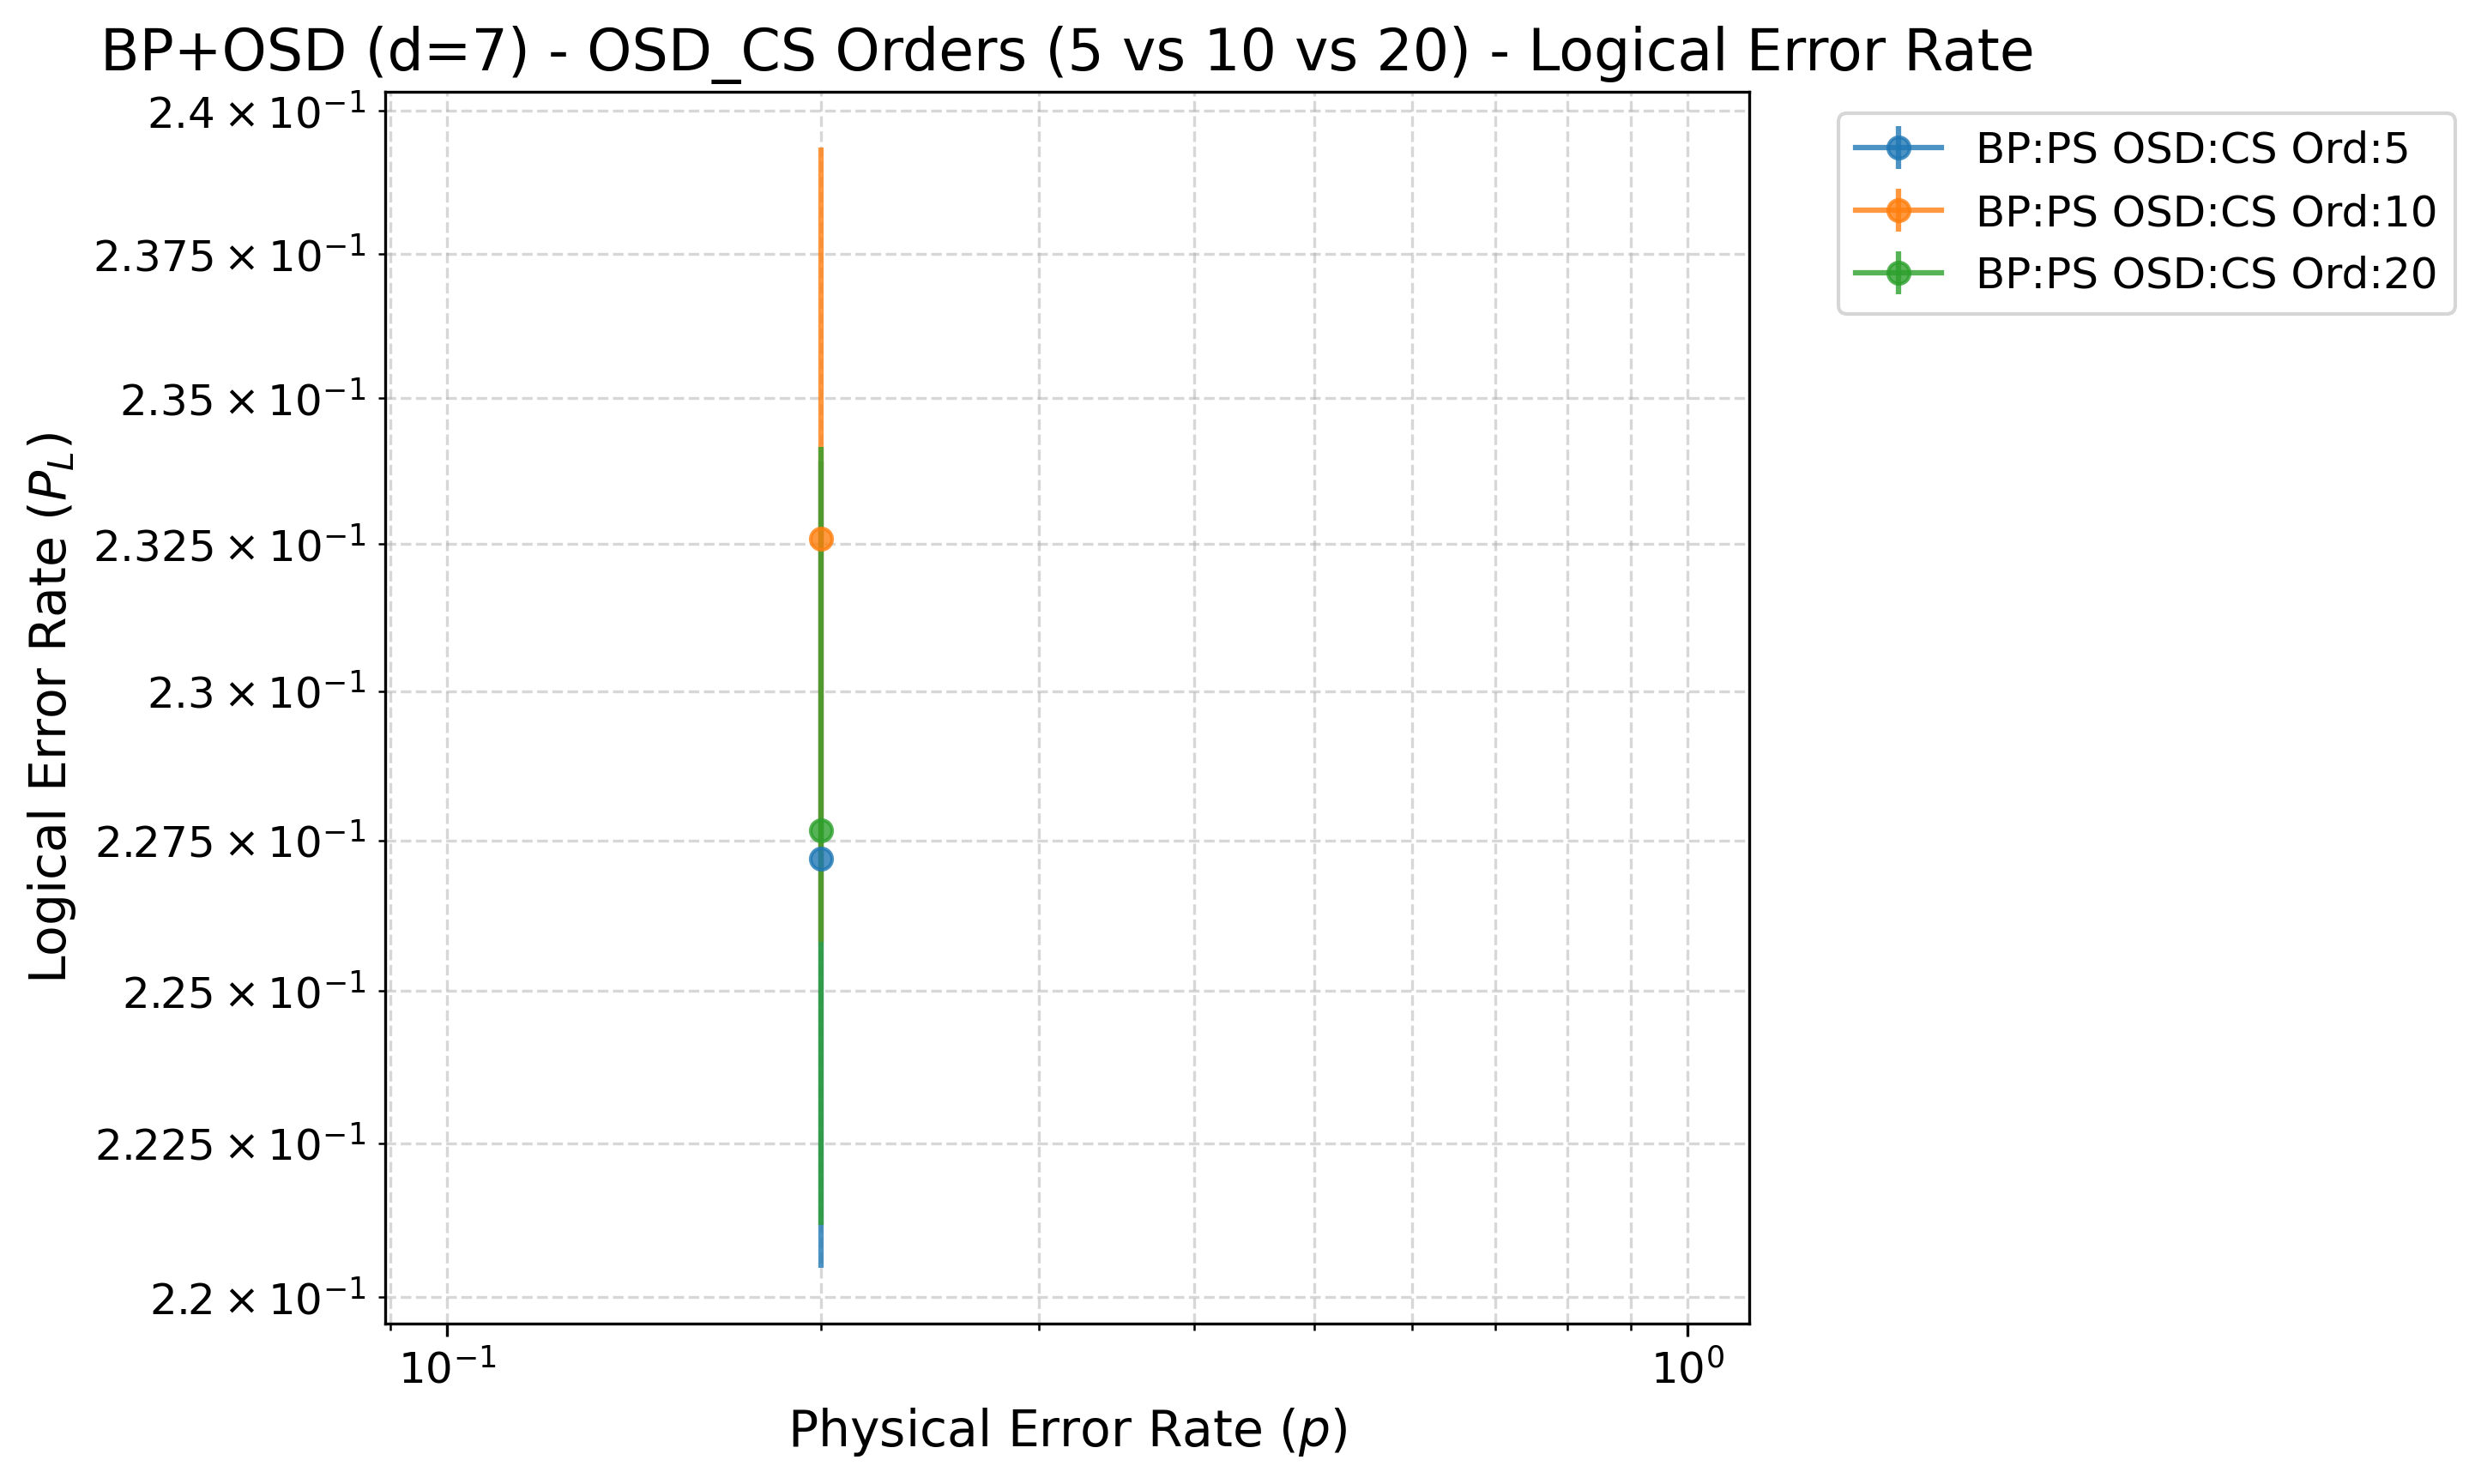
\includegraphics[width=\textwidth]{figures/chapter_6/s2b_bposd_osd_orders_error.png}
    \end{subfigure}
    \hfill
    \begin{subfigure}[b]{0.49\textwidth}
        \centering
        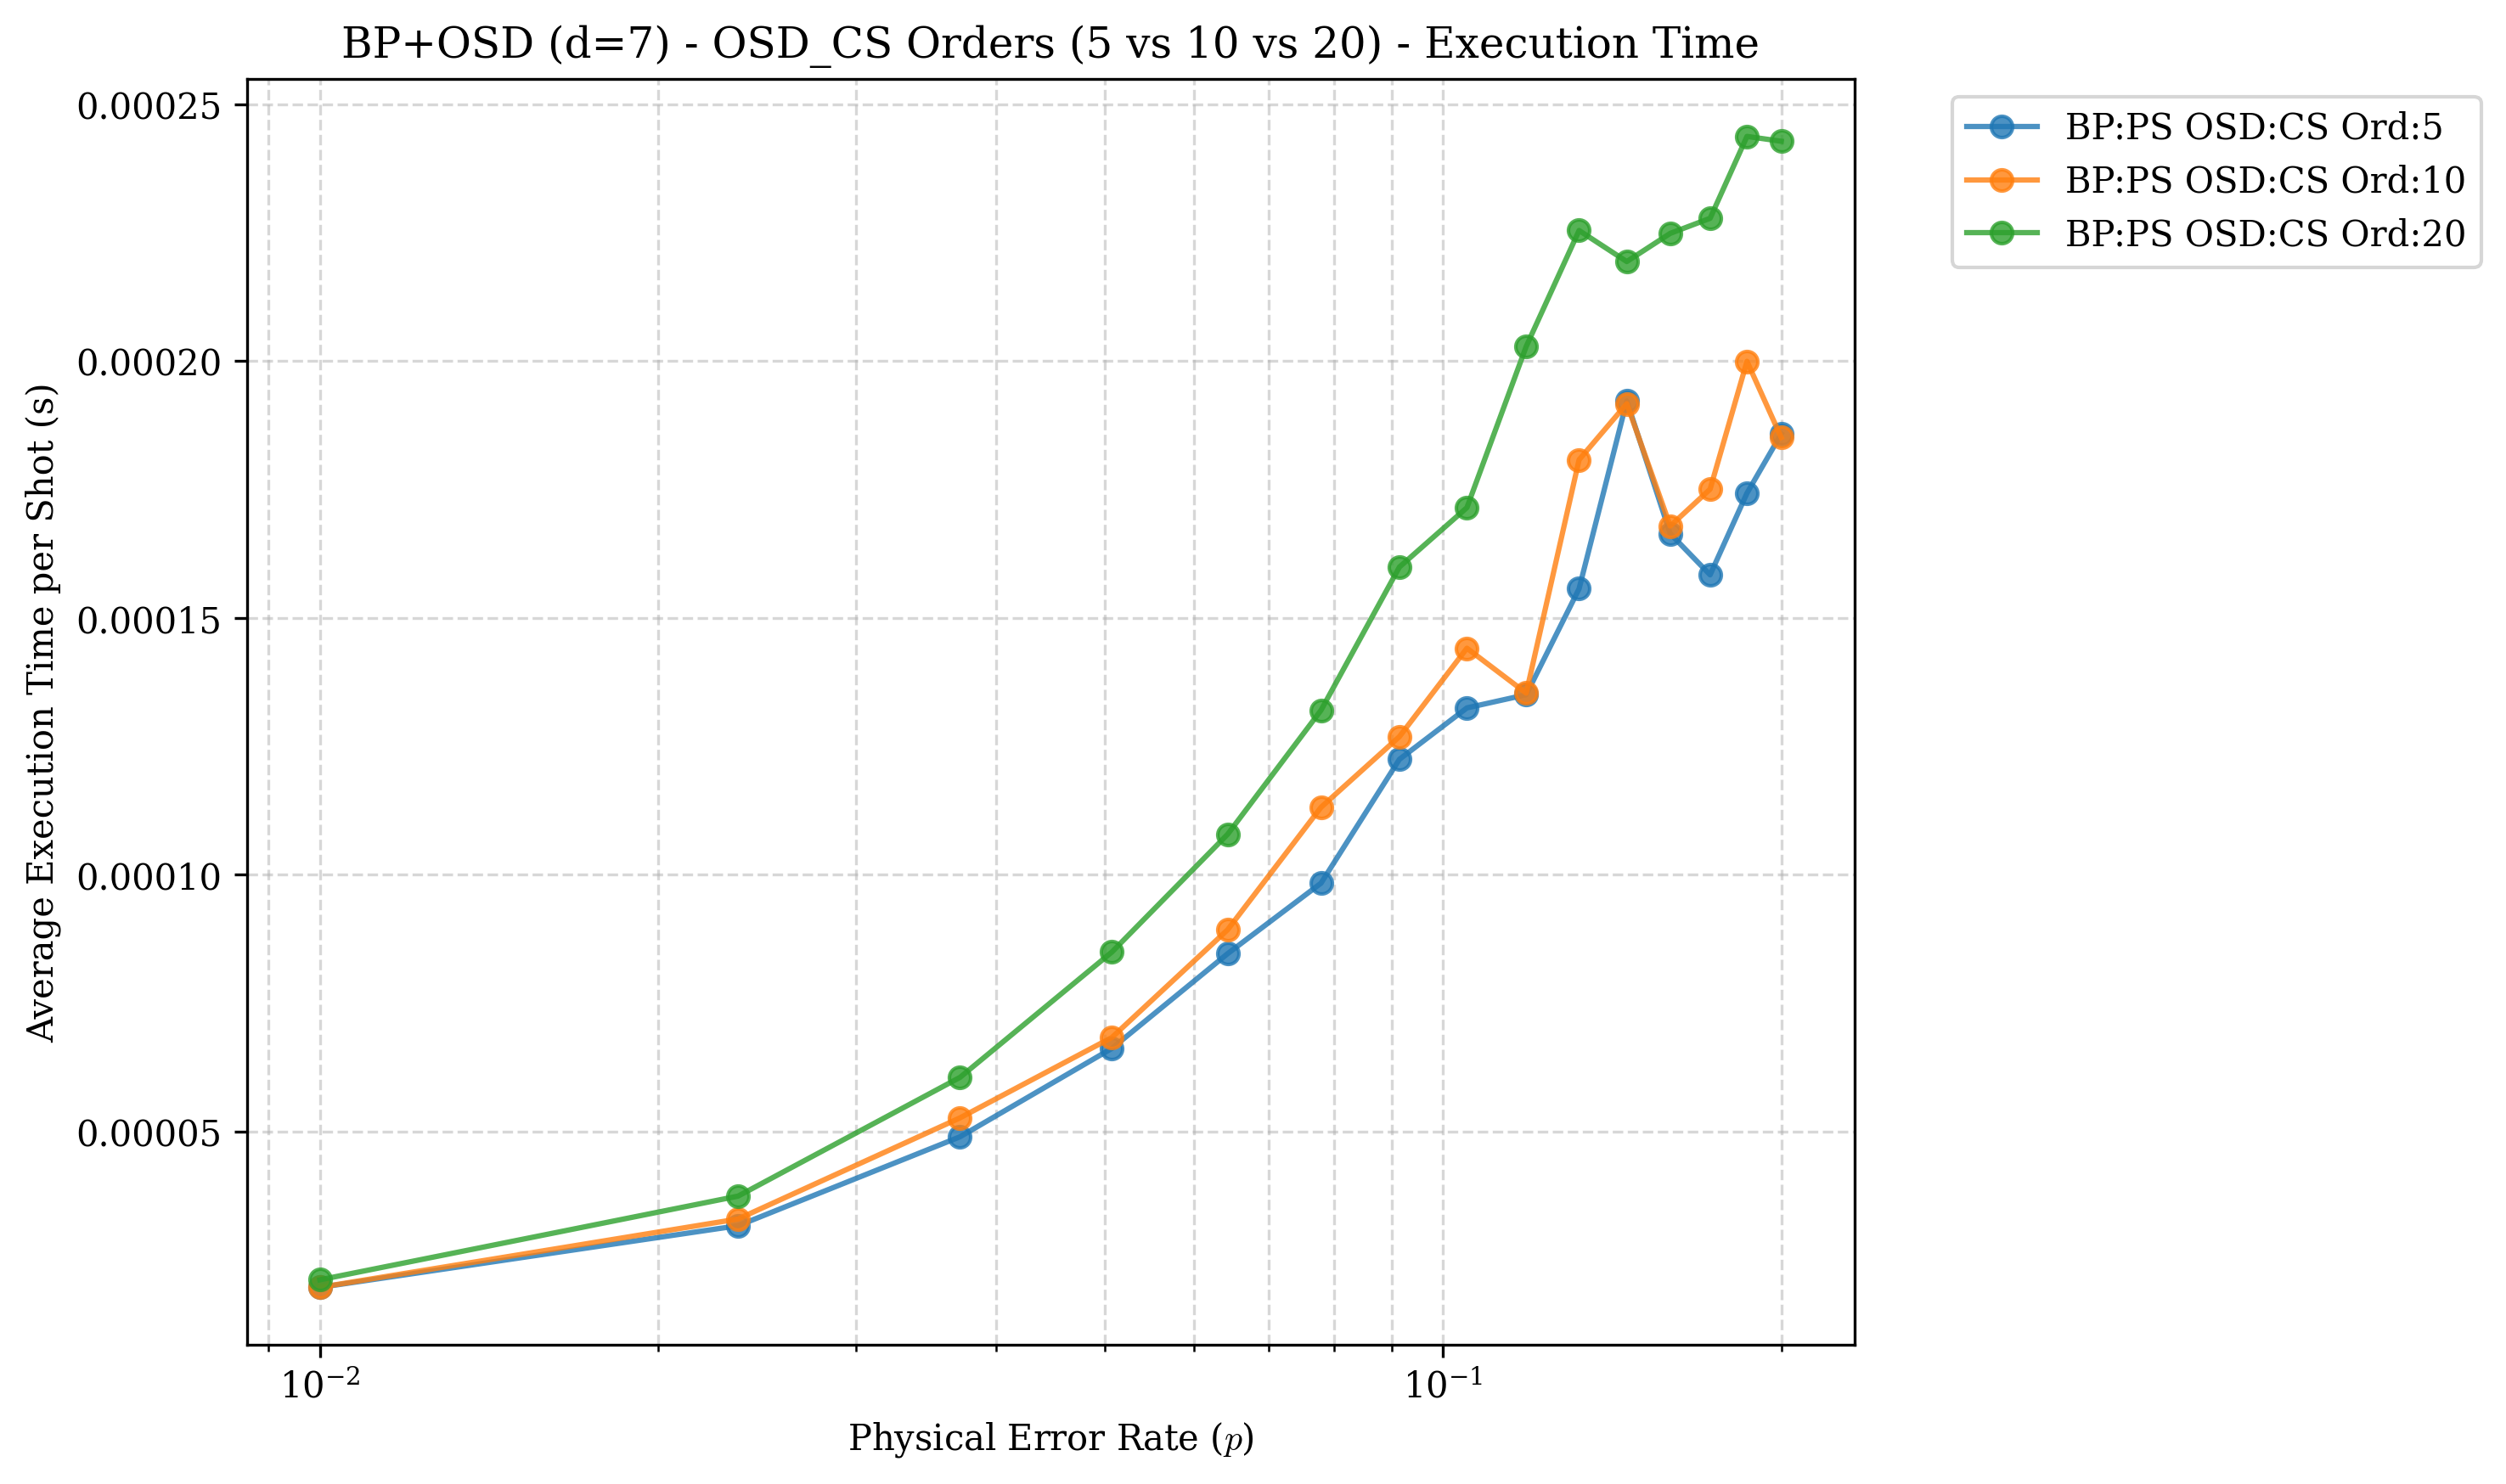
\includegraphics[width=\textwidth]{figures/chapter_6/s2b_bposd_osd_orders_time.png}
    \end{subfigure}
    \caption{Effect of the OSD search order ($k \in \{5, 10, 20\}$) on the logical error rate and execution time. An order of $k=10$ provides an optimal balance between accuracy and computational cost.}
    \label{fig:6:bposd_osd_orders}
\end{figure}

\subsection{Threshold Evaluation}
\label{subsec:6:bposd_threshold}

With the optimal parameters established (\textbf{BP Method:} MS, \textbf{OSD Method:} \texttt{osd\_cs}, \textbf{Order:} 10), we conducted a full Monte Carlo simulation to evaluate the algorithm's threshold on the 4.8.8 color code lattice. We evaluated distances from $d=3$ up to $d=11$. To guarantee robust statistics specially at low physical error rates, the simulation executed up to $20 \times 10^6$ shots per configuration, but stopping when $300$ logical errors have ocurred.

\notatfm{The threshold is calculated by interpolating the logical error curves for different distances and finding their crossing point, in a logarithmic representation.} The results of this simulation are presented in Figure \ref{fig:6:bposd_threshold}. The logical error rate curves cross at a threshold of $p_{th} \approx 14.32\%$. Below this crossing point, we observe a clear exponential suppression of the logical failure rate as the code distance increases, empirically proving the capability of the BP+OSD algorithm to effectively decode 2D Color Codes under a code-capacity noise model.

\begin{figure}[htbp]
    \centering
    \begin{subfigure}[b]{0.49\textwidth}
        \centering
        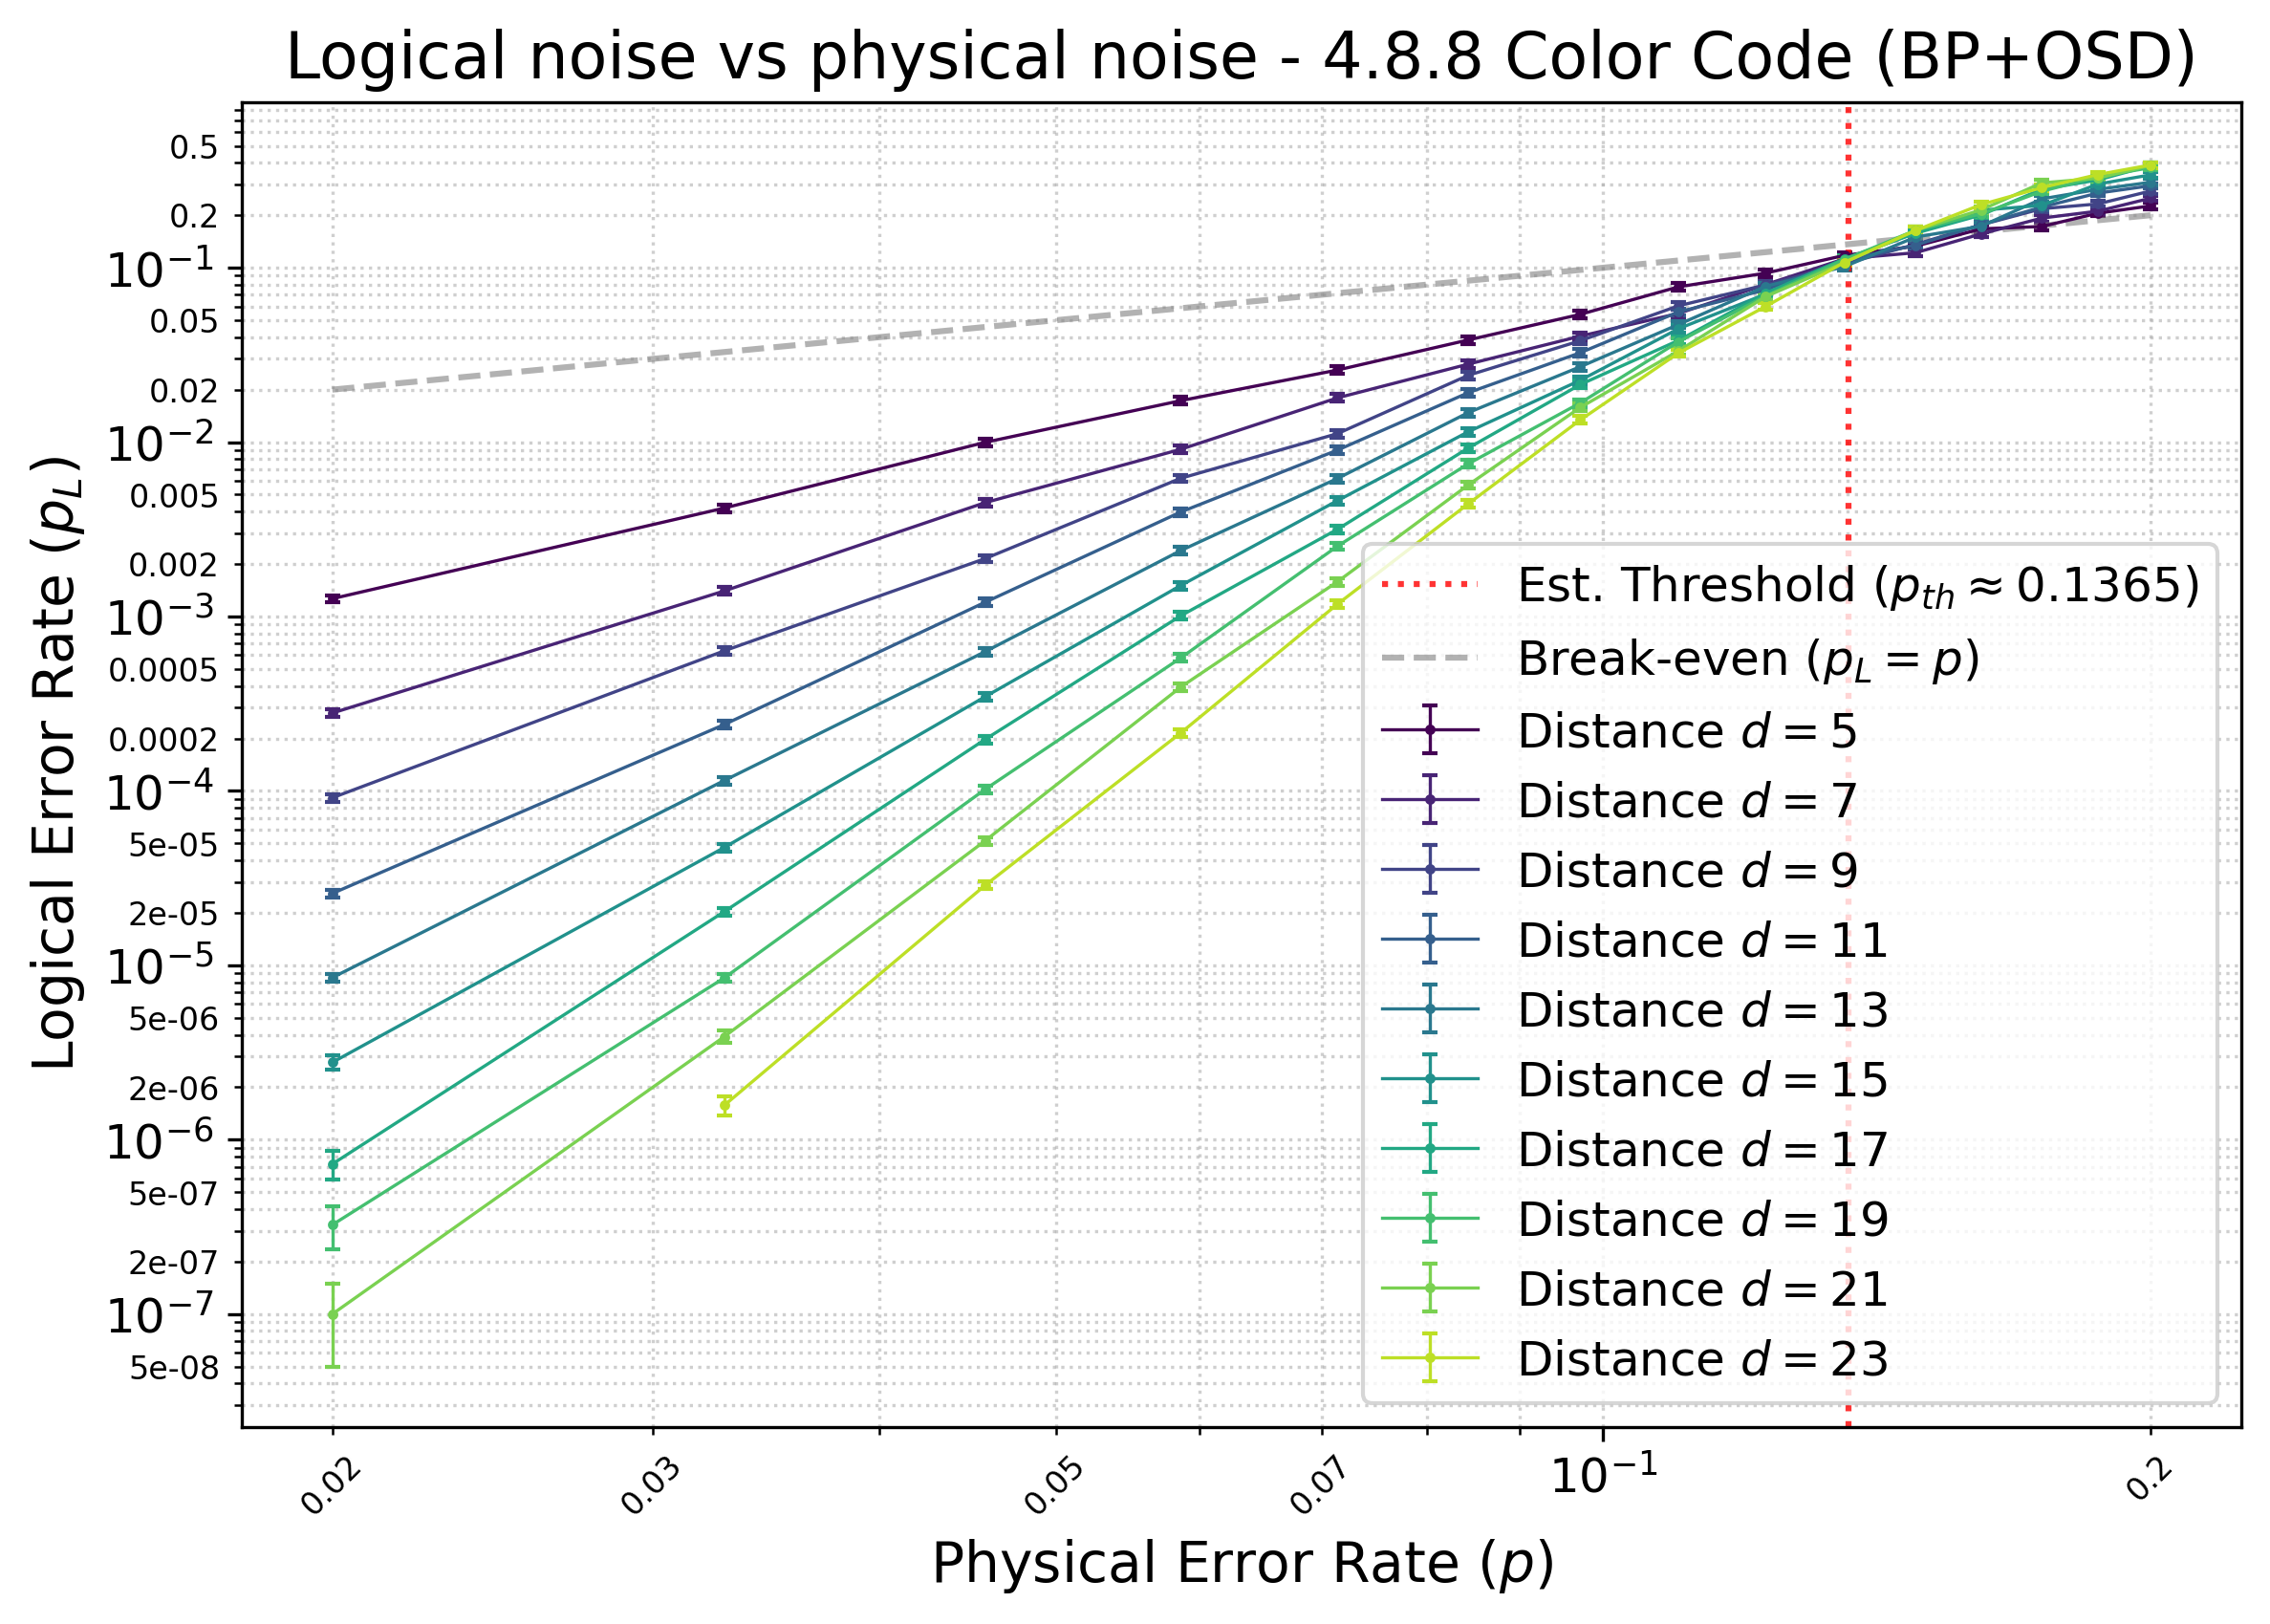
\includegraphics[width=\textwidth]{figures/chapter_6/s2_bposd_results_threshold.png}
    \end{subfigure}
    \hfill
    \begin{subfigure}[b]{0.49\textwidth}
        \centering
        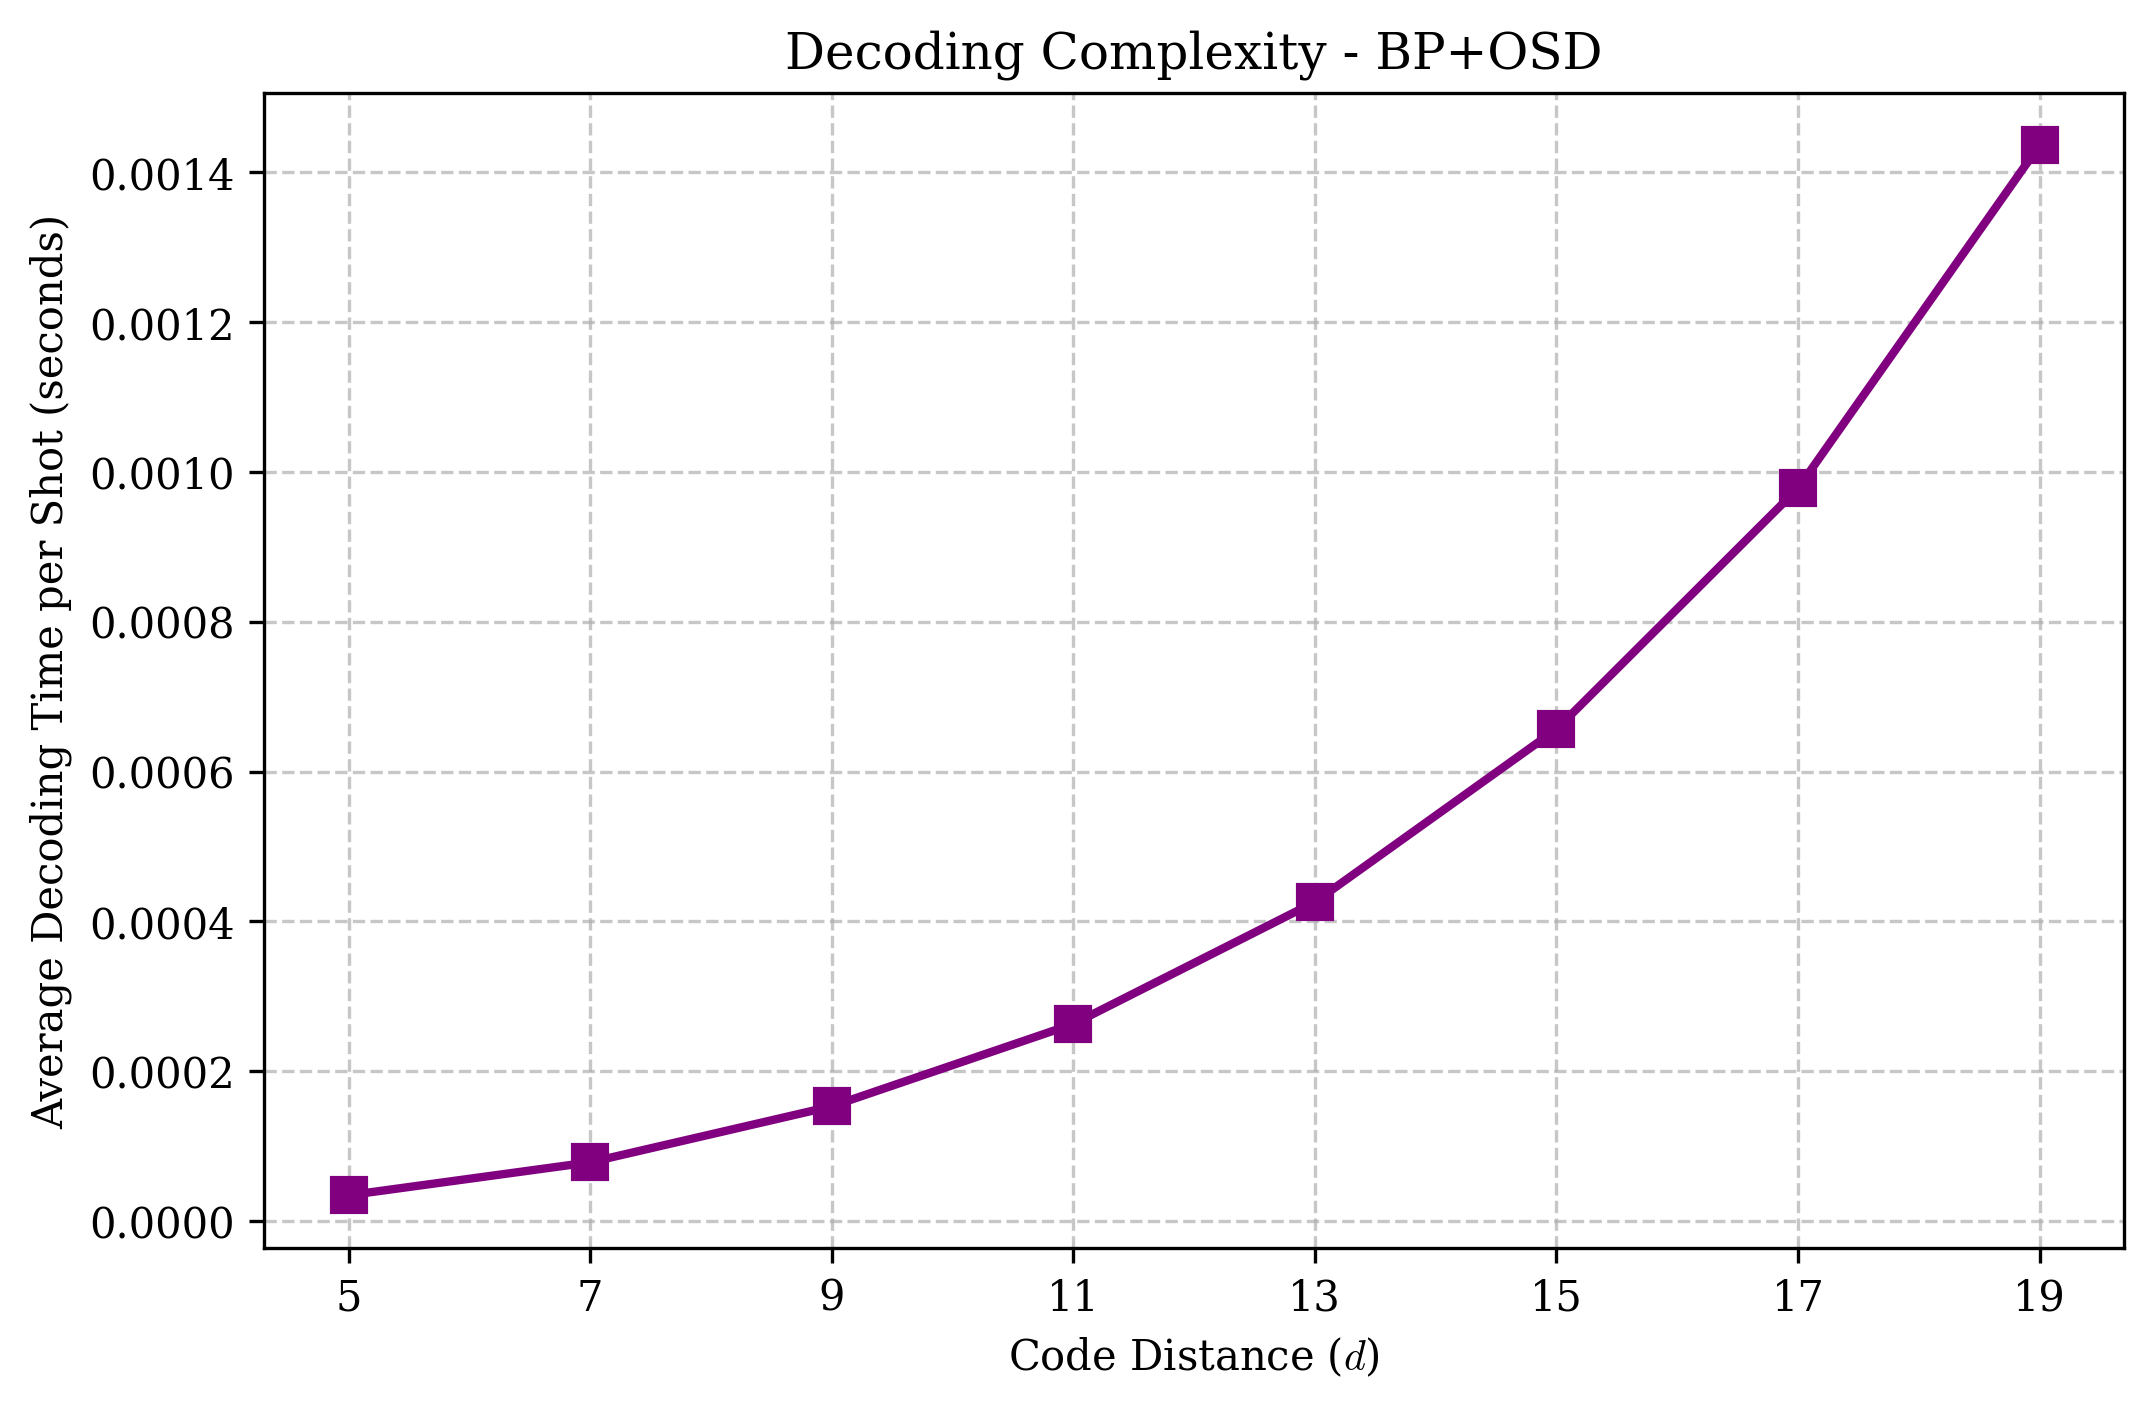
\includegraphics[width=\textwidth]{figures/chapter_6/s2_bposd_results_time.png}
    \end{subfigure}
    \caption{Simulation results for the configured BP+OSD decoder on the 4.8.8 Color Code lattice. The logical error threshold (left) is observed at $p_{th} \approx 14.32\%$. The corresponding average execution times per shot (right) confirm the expected behavior and polynomial scaling of the algorithm.}
    \label{fig:6:bposd_threshold}
\end{figure}



\section{Projection decoder + MWPM/Union-find}

\section{Restriction decoder + MWPM}

\section{Möbius Decoder + MWPM}

\section{Concatenated MWPM decoder}

\section{Correlated matching decoder}

